\documentclass[final]{beamer}
\mode<presentation>
{
  \usetheme{JDM}
}

\usepackage{multirow}
\usepackage{ragged2e}
\usepackage{times}
\usepackage{amsmath,amssymb}
\usepackage[english]{babel}
\usepackage[latin1]{inputenc}
\usepackage[orientation=landscape, size=custom, width=91, height=114, scale=1]{beamerposter}
\usepackage{array}
\usepackage{xspace}
\usepackage{xcolor}
\usepackage{epsfig}
\usepackage{caption}
\usepackage{subcaption}
\usepackage{booktabs}

\newcommand{\setblocksize}{\Large \centering}
\newcommand{\setsize}{\normalsize}
\newcommand{\paragraphbreak}{\vspace{1cm}}
\newcommand{\setfiguresize}{\normalsize}

\title{Jointly Improving Parsing and Perception for Natural Language Commands through Human-Robot Dialog}
\author{Jesse Thomason, Aishwarya Padmakumar, Jivko Sinapov, Nick Walker, Yuqian Jiang,\\Harel Yedidsion, Justin Hart, Peter Stone, and Raymond J. Mooney}
\institute{{\texorpdfstring{\color{blue} \bf \large}{ } Jesse Thomason},$^*$ Aishwarya Padmakumar,$^\dagger$ Jivko Sinapov,$^\ddagger$ Nick Walker,$^*$ Yuqian Jiang,$^\dagger$\\Harel Yedidsion,$^\dagger$ Justin Hart,$^\dagger$ Peter Stone,$^\dagger$ and Raymond J. Mooney$^\dagger$\\$^*$University of Washington;\\$^\dagger$University of Texas at Austin; $^\ddagger$Tufts University}

\date{\today}

\begin{document}
\setbeamertemplate{caption}{\raggedright\insertcaption\par}
%%%%%%%%%%%%%%%%%%%%%%%%%%%%%%%%%%%%%%%%%%%%%%%%%%%%%%%%%%%%%%%%%%%%%%%%%%%%%%%%%%%%%%%%%%%
\begin{frame}{} 
  \vfill
  
%\vspace{-270pt}  %added here to get it closer to top...
\begin{columns}[t]

%%%%%%%%%%%%%%%%%%%%%%%%%%%%%%%%%%%%%%%%%%%%%%%%%%%%%%%%%%%%%%%%%%%%%%%%%%%%%%%%%%%%%%%%%%%
\begin{column}{.24\linewidth}    %%% COLUMN 1 %%%

\begin{block}{\setblocksize Learning via Human-Robot Dialog}
%\vspace{-30pt}
	\vspace{1mm}
\justifying{\setsize
Natural language understanding for robotics can require substantial domain- and platform-specific engineering.
One way to alleviate engineering for a new domain is to enable robots in human environments to adapt dynamically---continually learning new language constructions and perceptual concepts.
We present an end-to-end pipeline for translating natural language commands to robot actions, and use clarification dialogs to jointly improve parsing and concept grounding.

\begin{figure}
\centering
  \begin{subfigure}{0.9\textwidth}
    \centering
    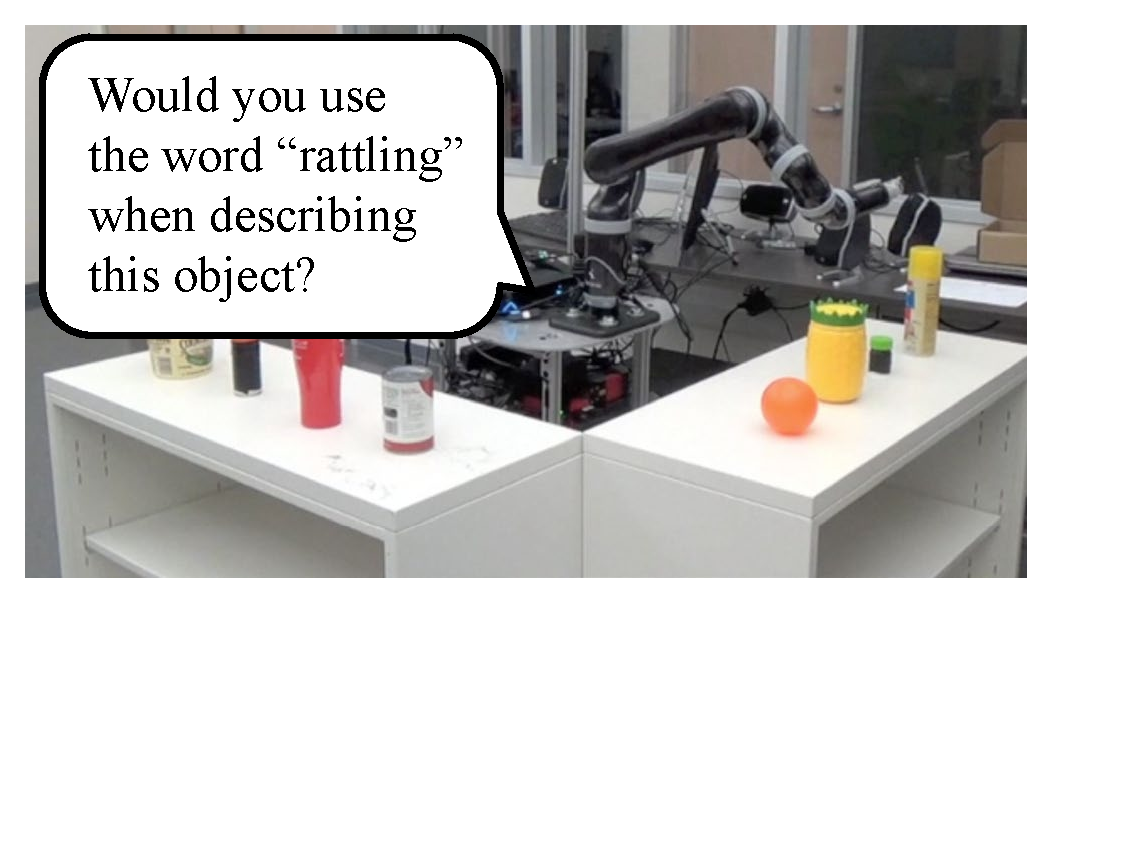
\includegraphics[width=\linewidth]{figures/rattling_ask.pdf}
    \vspace{-4cm}
  \end{subfigure}
  \begin{subfigure}{0.92\textwidth}
    \centering
    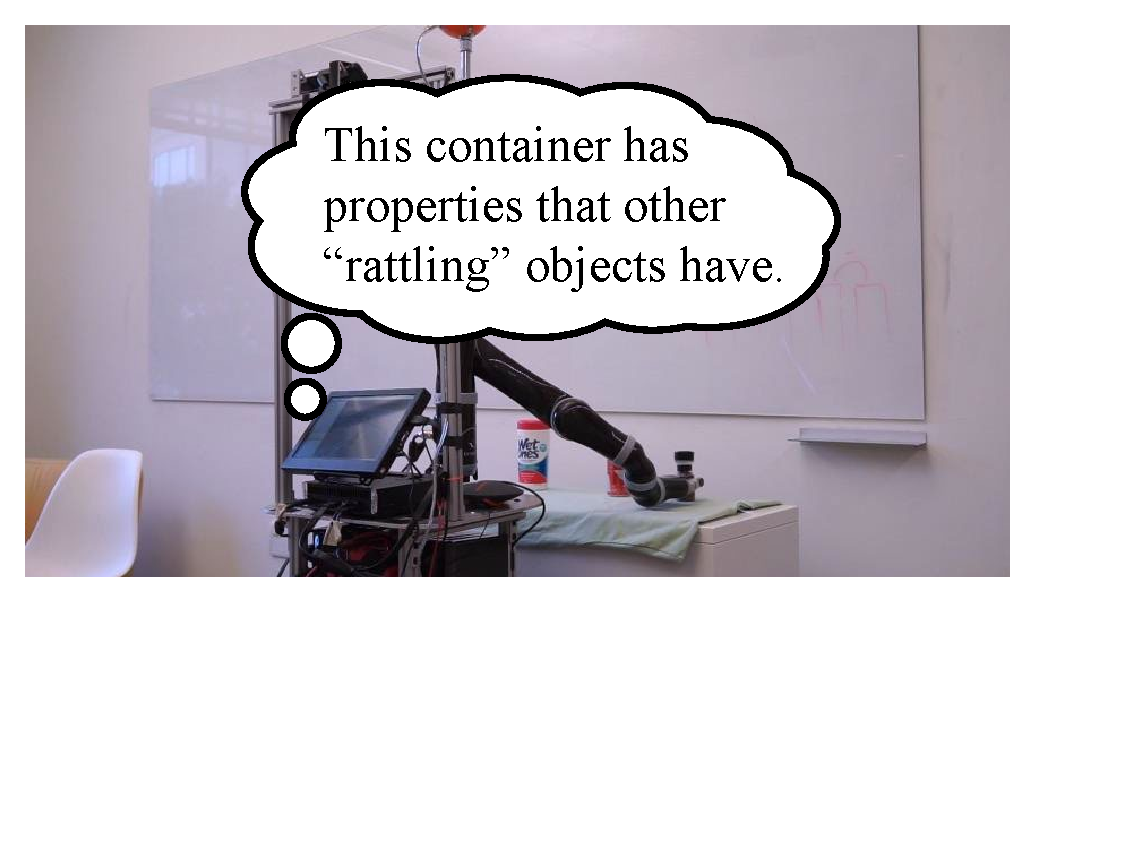
\includegraphics[width=\linewidth]{figures/rattling_think.pdf}
    \vspace{-4cm}
  \end{subfigure}
\end{figure}
Through dialog, a robot agent can acquire task-relevant information from a human on the fly.
Here, \emph{rattling} is a new concept the agent learns with human guidance in order to pick out a remote target object later on.
\paragraphbreak

\begin{figure}
\centering
  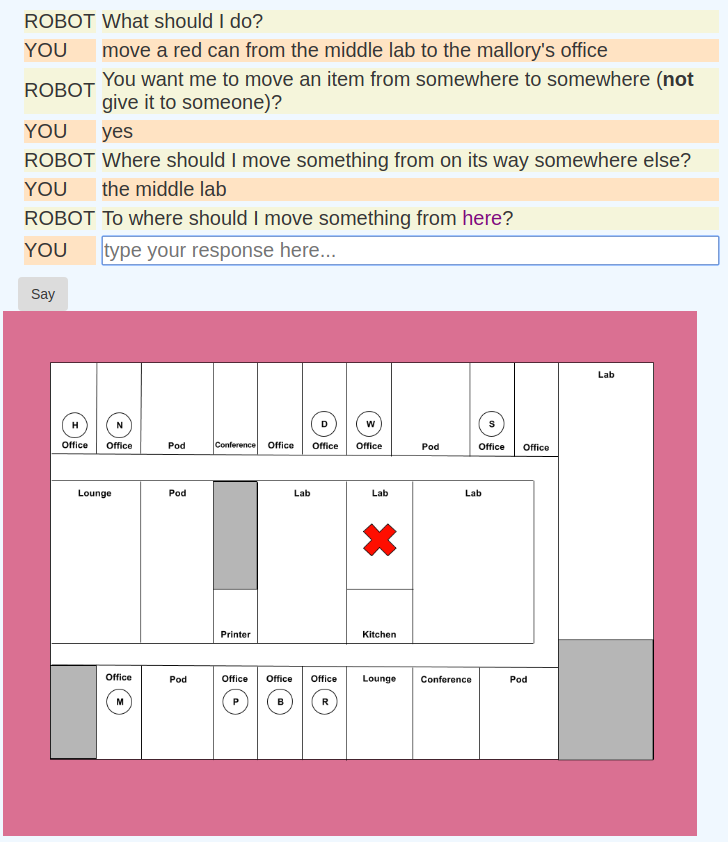
\includegraphics[width=1\linewidth]{figures/interface_move_example.png}
  \label{fig:phm_web_interface_move}
\end{figure}

We train the agent in simulation with real human users on Mechanical Turk.
The user gives a command to the learning agent, and the agent replies with questions to clarify the command.
Each clarification generates a new training example for the agent's semantic parser, enabling retraining from conversational data.
\paragraphbreak

\begin{figure}
\centering
  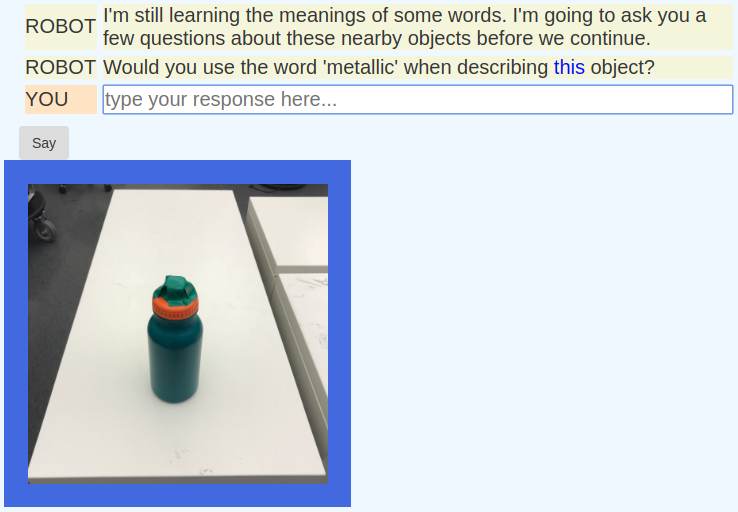
\includegraphics[width=1\linewidth]{figures/interface_oal_yn_ex.png}
  \label{fig:web_interface_oal}
\end{figure}

In addition to asking for semantic clarifications, the agent can ask whether a concept word applies to a specific object, and for examples.
Learning these models while retraining the semantic parser connects words to concept models corresponding to physical properties of objects like color, weight, and sound.

}
\end{block}

\end{column}	%%% END COLUMN 1 %%%

%%%%%%%%%%%%%%%%%%%%%%%%%%%%%%%%%%%%%%%%%%%%%%%%%%%%%%%%%%%%%%%%%%%%%%%%%%%%%%%%%%%%%%%%%%%
\begin{column}{.49\linewidth}    %%% COLUMN 2 %%%

\begin{block}{\setblocksize }
%\vspace{-30pt}
  \vspace{1mm}
\justifying{\Huge
Asking questions can help a robot understand compositional language and grounded word meanings during human-robot dialogs.
}
\paragraphbreak

{\Large
Talk to the agent! \url{https://bit.ly/2W3jiJP}.
}
\end{block}

\begin{block}{\setblocksize }
%\vspace{-30pt}
  \vspace{1mm}
\justifying{\setsize

\begin{figure}[ht]
\centering
  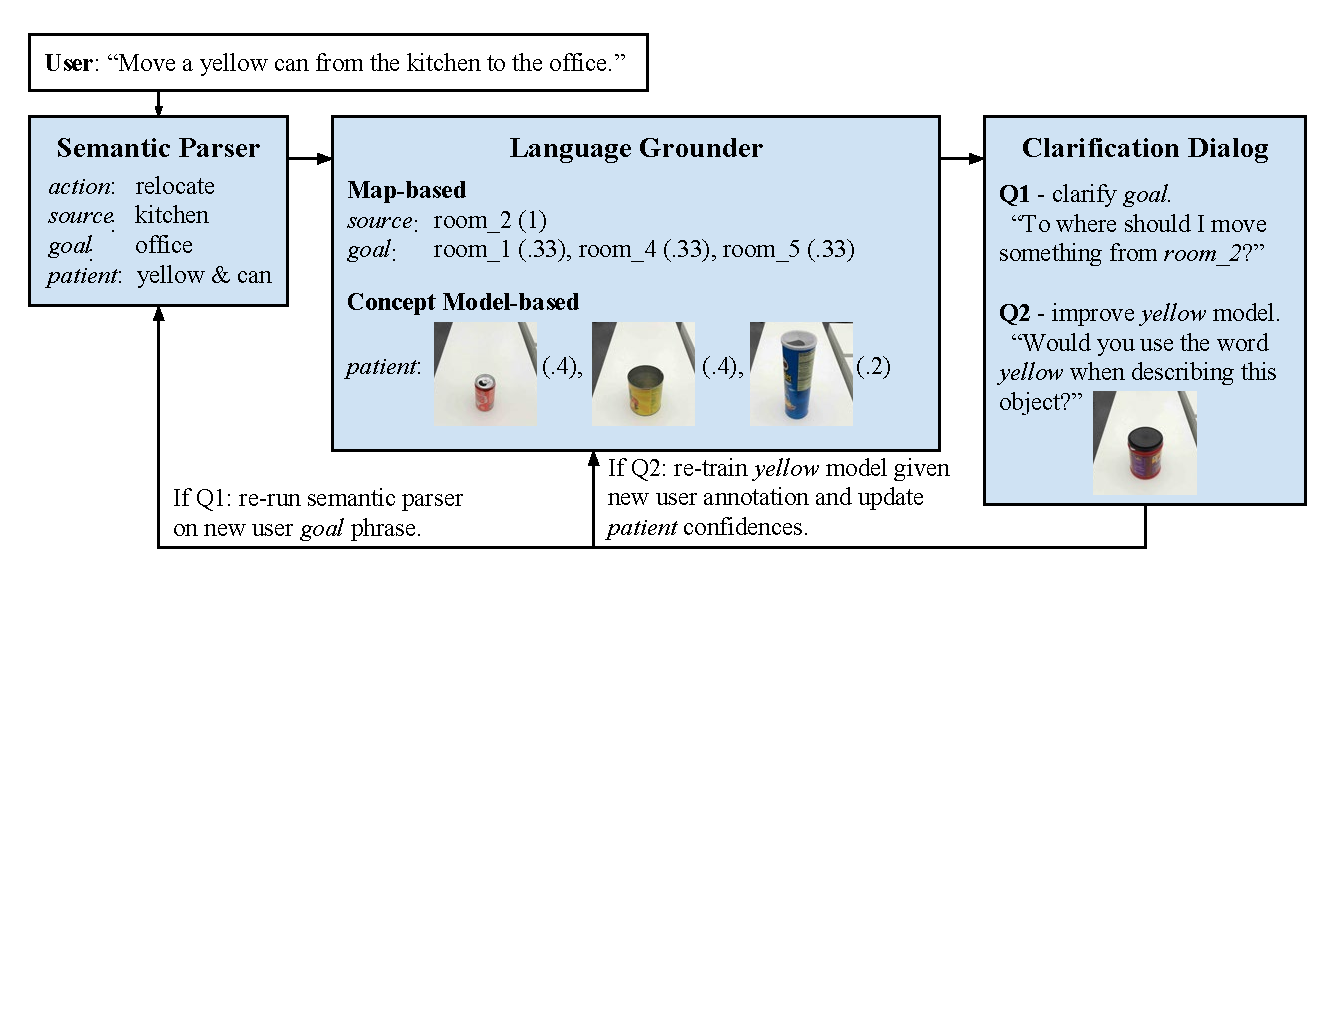
\includegraphics[width=1\linewidth]{figures/agent_components_fig.pdf}
  \vspace{-15cm}
\end{figure}

User commands are parsed into semantic slots ({\bf left}), which are grounded ({\bf center}) using either a known map (for rooms and people) or learned concept models (for objects) to a distribution over possible satisfying constants (e.g., all rooms that can be described as an ``office'').
A clarification dialog ({\bf right}) is used to recover from ambiguous or misunderstood slots (e.g., {\it Q1}), and to improve concept models on the fly (e.g., {\it Q2}).
\paragraphbreak

\begin{figure}
\centering
\begin{subfigure}{1.\textwidth}
  \centering
  {\large
  \begin{tabular}{cc}
    \begin{tabular}{ll}
      \textcolor{red}{\textbf{R}}:& \textcolor{red}{What should I do?} \\
      \textcolor{blue}{\textbf{H}}:& \textcolor{blue}{Move a rattling container from the} \\
      & \textcolor{blue}{lounge by the conference room to} \\
      & \textcolor{blue}{Bob's office.} \\
      \textcolor{red}{\textbf{R}}:& \textcolor{red}{Does rattling refer to a property of} \\
      & \textcolor{red}{an object?} \\
      \textcolor{blue}{\textbf{H}}:& \textcolor{blue}{Yes.} \\
      \textcolor{red}{\textbf{R}}:& \textcolor{red}{Does rattling mean the same thing} \\
      & \textcolor{red}{as empty?} \\
      \textcolor{blue}{\textbf{H}}:& \textcolor{blue}{No.} \\
      \textcolor{red}{\textbf{R}}:& \textcolor{red}{I am still learning the meanings of} \\
      & \textcolor{red}{some words.} \\
      \textcolor{red}{\textbf{R}}:& \textcolor{red}{Show me an object you could use} \\
      & \textcolor{red}{the word rattling when describing,} \\
      & \textcolor{red}{or say ``none of them.''} \\
      \textcolor{blue}{\textbf{H}}:& \textcolor{blue}{Watch.} \\
      \textcolor{red}{\textbf{R}}:& \textcolor{red}{I am getting the objects on the table} \\
      & \textcolor{red}{into focus$\dots$ Okay, I see them.} \\
      \textcolor{blue}{\textbf{H}}:& \textcolor{blue}{This one. \emph{The human picks up a}} \\
      & \textcolor{blue}{\emph{small, full pill jar.}} \\
    \end{tabular} &
    \begin{tabular}{ll}
      \textcolor{red}{\textbf{R}}:& \textcolor{red}{I see.} \\
      \textcolor{red}{\textbf{R}}:& \textcolor{red}{Show me an object you could not} \\
      & \textcolor{red}{use the word rattling when} \\
      & \textcolor{red}{describing, or say ``all of them.''} \\
      \textcolor{blue}{\textbf{H}}:& \textcolor{blue}{Watch. This one. \emph{The human picks}} \\
      & \textcolor{blue}{\emph{up a red water bottle.}} \\
      \textcolor{red}{\textbf{R}}:& \textcolor{red}{I see.} \\
      \textcolor{red}{\textbf{R}}:& \textcolor{red}{Show me an object you could use} \\
      & \textcolor{red}{the word rattling when describing,} \\
      & \textcolor{red}{or say ``none of them.''} \\
      \textcolor{blue}{\textbf{H}}:& \textcolor{blue}{Watch. This one. \emph{The human picks}} \\
      & \textcolor{blue}{\emph{up a container half-full of beans.}} \\
      \textcolor{red}{\textbf{R}}:& \textcolor{red}{I see.} \\
      \textcolor{red}{\textbf{R}}:& \textcolor{red}{Thanks. Now back to business.} \\
      \textcolor{red}{\textbf{R}}:& \textcolor{red}{You want me to move an item} \\
      & \textcolor{red}{from 3.514 to somewhere?} \\
      \textcolor{blue}{\textbf{H}}:& \textcolor{blue}{Yes.} \\
      \textcolor{red}{\textbf{R}}:& \textcolor{red}{I should move something from} \\
      & \textcolor{red}{3.514 to 3.510?} \\
      \textcolor{blue}{\textbf{H}}:& \textcolor{blue}{Yes.}
    \end{tabular}
  \end{tabular}
  }
  \label{fig:segbot_demo:conv}
\end{subfigure}
\begin{subfigure}{0.4\textwidth}
  \centering
  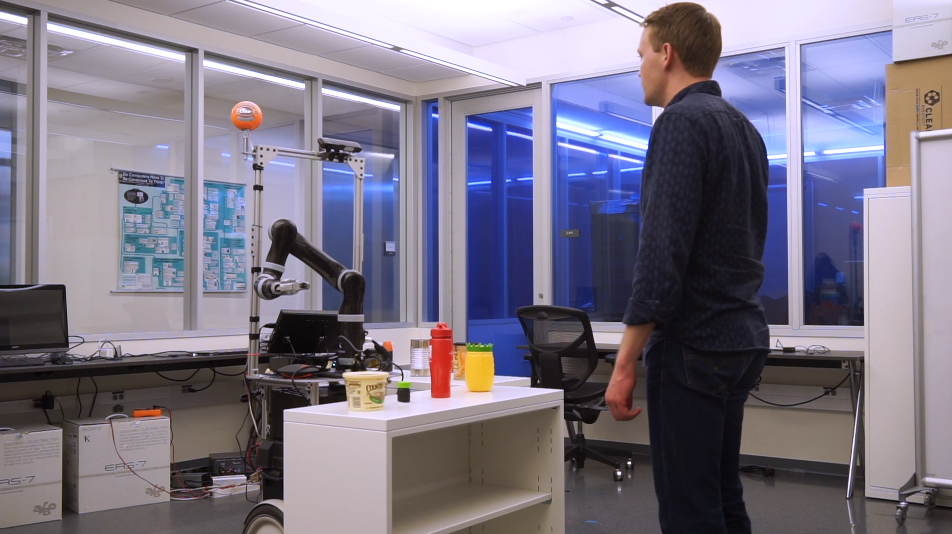
\includegraphics[width=\linewidth]{figures/demo_1.png}
  \caption{\setsize The human says novel word \emph{rattling}.}
\end{subfigure}
\begin{subfigure}{0.4\textwidth}
  \centering
  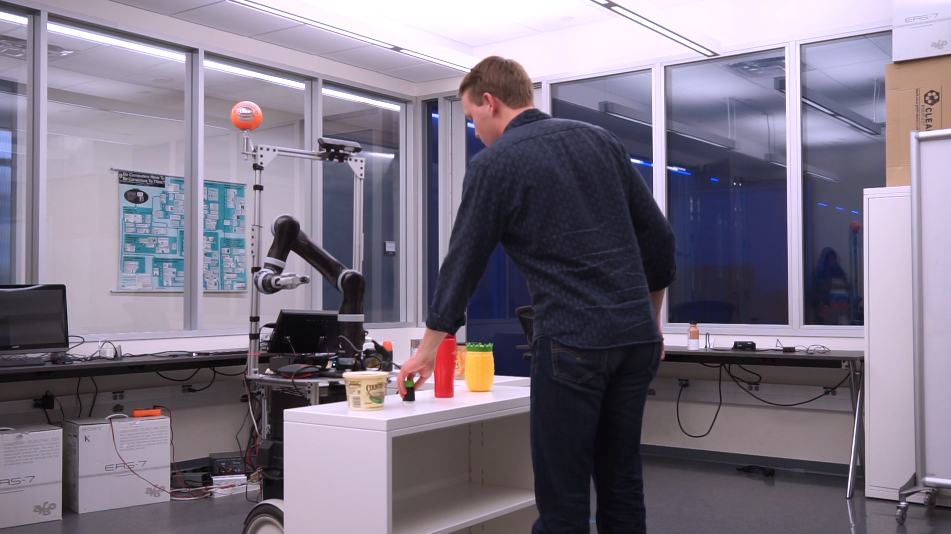
\includegraphics[width=\linewidth]{figures/demo_2.png}
  \caption{\setsize The robot learns what \emph{rattling} means.}
\end{subfigure}
\begin{subfigure}{0.4\textwidth}
  \centering
  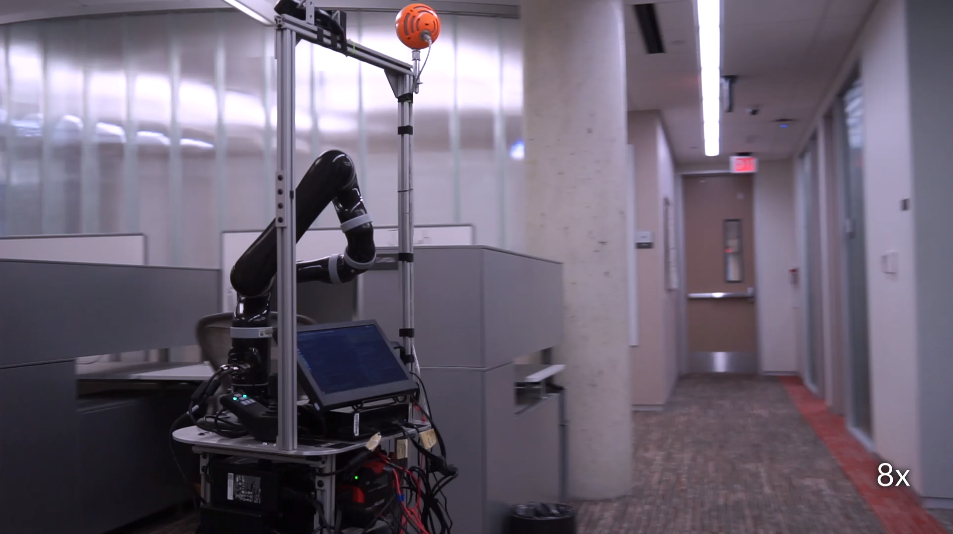
\includegraphics[width=\linewidth]{figures/demo_3.png}
  \caption{\setsize The robot navigates to the \emph{source} room.}
\end{subfigure}
\begin{subfigure}{0.4\textwidth}
  \centering
  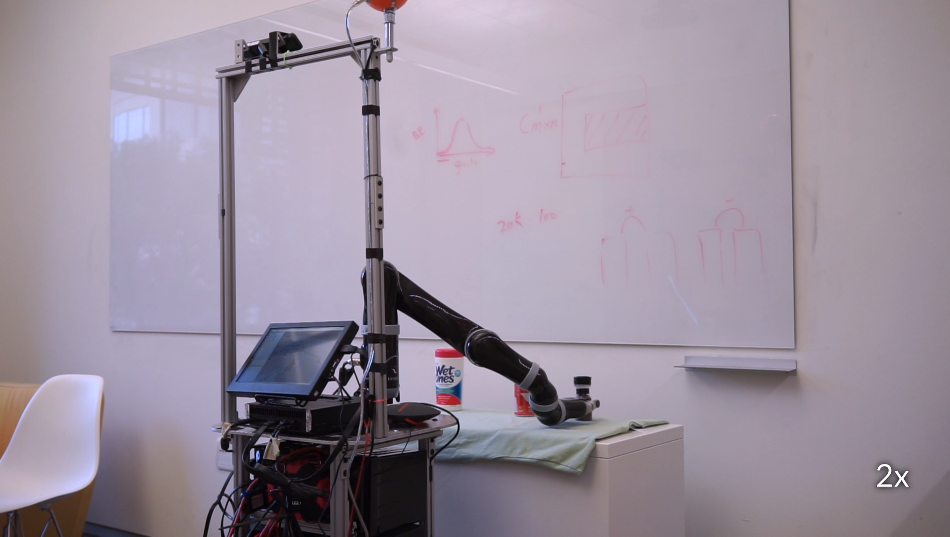
\includegraphics[width=\linewidth]{figures/demo_4.png}
  \caption{\setsize The robot grasps a \emph{rattling container}.}
\end{subfigure}
\begin{subfigure}{0.4\textwidth}
  \centering
  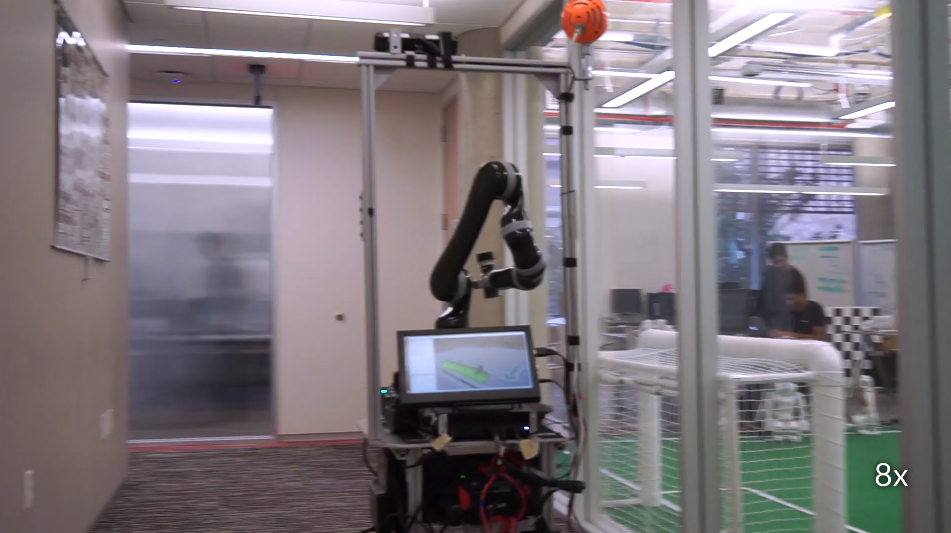
\includegraphics[width=\linewidth]{figures/demo_5.png}
  \caption{\setsize The robot navigates to the \emph{goal} room.}
\end{subfigure}
\begin{subfigure}{0.4\textwidth}
  \centering
  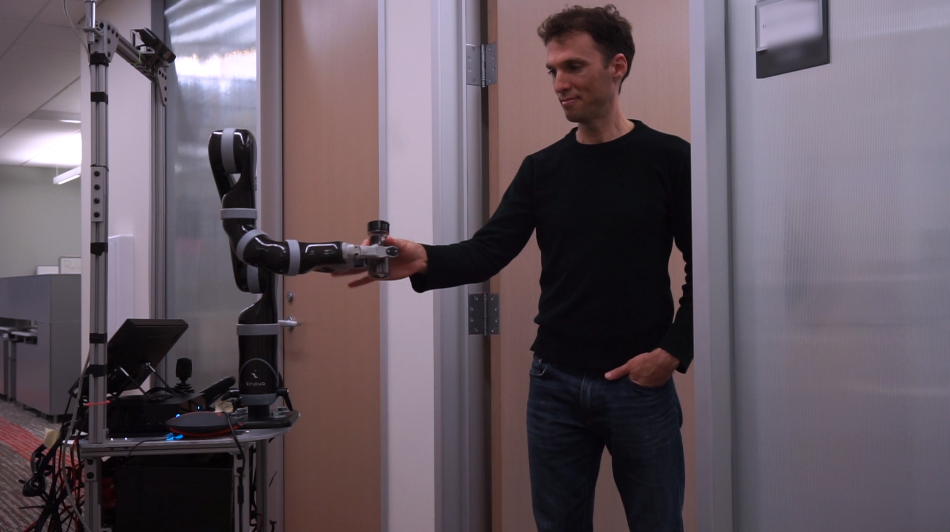
\includegraphics[width=\linewidth]{figures/demo_6.png}
  \caption{\setsize The robot hands over the \emph{patient} item.}
\end{subfigure}
  \label{fig:segbot_demo}
\end{figure}
\vspace{3mm}

The robot learns a new word, \emph{rattling}, which requires auditory perception, and is then able to navigate to the specified room, identify a \emph{rattling container} item, and deliver the item to the specified destination.

}
\end{block}

\end{column}  %%% END COLUMN 2 %%%

%%%%%%%%%%%%%%%%%%%%%%%%%%%%%%%%%%%%%%%%%%%%%%%%%%%%%%%%%%%%%%%%%%%%%%%%%%%%%%%%%%%%%%%%%%%
\begin{column}{0.24\linewidth}    %%% COLUMN 3 %%%

\begin{block}{\setblocksize Mechanical Turk Evaluation}
%\vspace{-30pt}
	\vspace{1mm}
\justifying{\setsize

After training on batches of dialogs with users on a set of training tasks, we test agents against unseen test tasks.
We compare an {\it Initial} agent against one with a \emph{Trained}$^*$ \emph{Perception} module, and one with \emph{Trained} \emph{Parsing} and \emph{Perception} modules.
We measure the number of clarification questions asked during the dialog.
This metric should decrease as the agent refines its parsing and perception modules, needing to ask fewer questions about the unseen locations and objects in the test tasks.
We also compare users' answers to usability questions answered on a 7-point Likert scale: from \emph{Strongly Disagree} (1) to \emph{Strongly Agree} (7).

\begin{table}[t]
    \centering
    \begin{tabular}{l r r r}
        \multirow{2}{*}{$\mathcal{A}$} & \multicolumn{3}{c}{Clarification Questions $\downarrow$} \\
        & \multicolumn{1}{c}{Navigation $(p)$} & \multicolumn{1}{c}{Delivery $(p)$} & \multicolumn{1}{c}{Relocation $(p)$} \\
        \toprule
        In & $3.02\pm6.48$\phantom{$(.00)$} & $6.81\pm8.69$\phantom{$(.00)$} & $22.3\pm9.15$\phantom{$(.00)$} \\
        Tr$^*$ & $4.05\pm8.81 (.46)$ & $8.16\pm13.8 (.53)$ & $23.5\pm6.07 (.67)$ \\
        Tr & $1.35\pm4.44 (.11)$ & $7.50\pm9.93 (.72)$ & $19.6\pm7.89 (.47)$ \\
        \bottomrule
    \end{tabular}
\end{table}
The average number of clarification questions agents asked among successful dialogs.
Also given are the $p$-values of a Welch's $t$-test between the \textbf{Tr}\emph{ained}$^*$ (\emph{Perception}) and \textbf{Tr}\emph{ained} (\emph{Parsing+Perception}) model ratings against the \textbf{In}\emph{itial} model ratings.
\paragraphbreak

For both \emph{navigation} and \emph{relocation}, there is a slight decrease in the number of questions between the \emph{Initial} agent and the \emph{Trained (Parsing+Perception)} agent.
The \emph{Trained (Perception)} agent sees slightly worse performance across tasks, possibly due to a larger lexicon of adjectives and nouns (e.g., \emph{can} as a descriptive noun now polysemous with \emph{can} as a verb---\emph{can you...}) without corresponding parsing updates.

\begin{table}[t]
    \centering
    \begin{tabular}{l r r r}
        \multirow{2}{*}{$\mathcal{A}$} & \multicolumn{3}{c}{Usability Survey (Likert 1-7) $\uparrow$} \\
        & \multicolumn{1}{c}{Navigation $(p)$} & \multicolumn{1}{c}{Delivery $(p)$} & \multicolumn{1}{c}{Relocation $(p)$} \\
        \toprule
        In & $3.09\pm2.04$\phantom{$(.00)$} & $3.20\pm2.12$\phantom{$(.00)$} & $3.37\pm2.17$\phantom{$(.00)$} \\
        Tr$^*$ & $3.51\pm2.05 (.09)$ & $3.60\pm2.09 (.12)$ & $3.60\pm2.08 (.37)$ \\
        Tr & $\pmb{3.76}\pm2.07 (.01)$ & $\pmb{3.87}\pm2.10 (.01)$ & $\pmb{3.93}\pm2.16 (.04)$ \\
        \bottomrule
    \end{tabular}
\end{table}
The average Likert rating given on usability survey prompts for each task across the agents.
{\bf Bold} indicates an average \textbf{Tr}\emph{ained}$^*$ (\emph{Perception}) and \textbf{Tr}\emph{ained} (\emph{Parsing+Perception}) model ratings significantly higher than the \textbf{In}\emph{itial} model ($p<0.05$) under a Welch's $t$-test.
\paragraphbreak

Across tasks, the \emph{Trained (Parsing+Perception)} agent is rated as more usable than both the \emph{Initial} agent and the \emph{Trained (Perception)} agent that updated only its concept models from training conversations.

\begin{figure}
\centering
\begin{tabular}[t!]{ccc}
  \multicolumn{3}{c}{\bf Learned Concept Model for \emph{can}} \\
  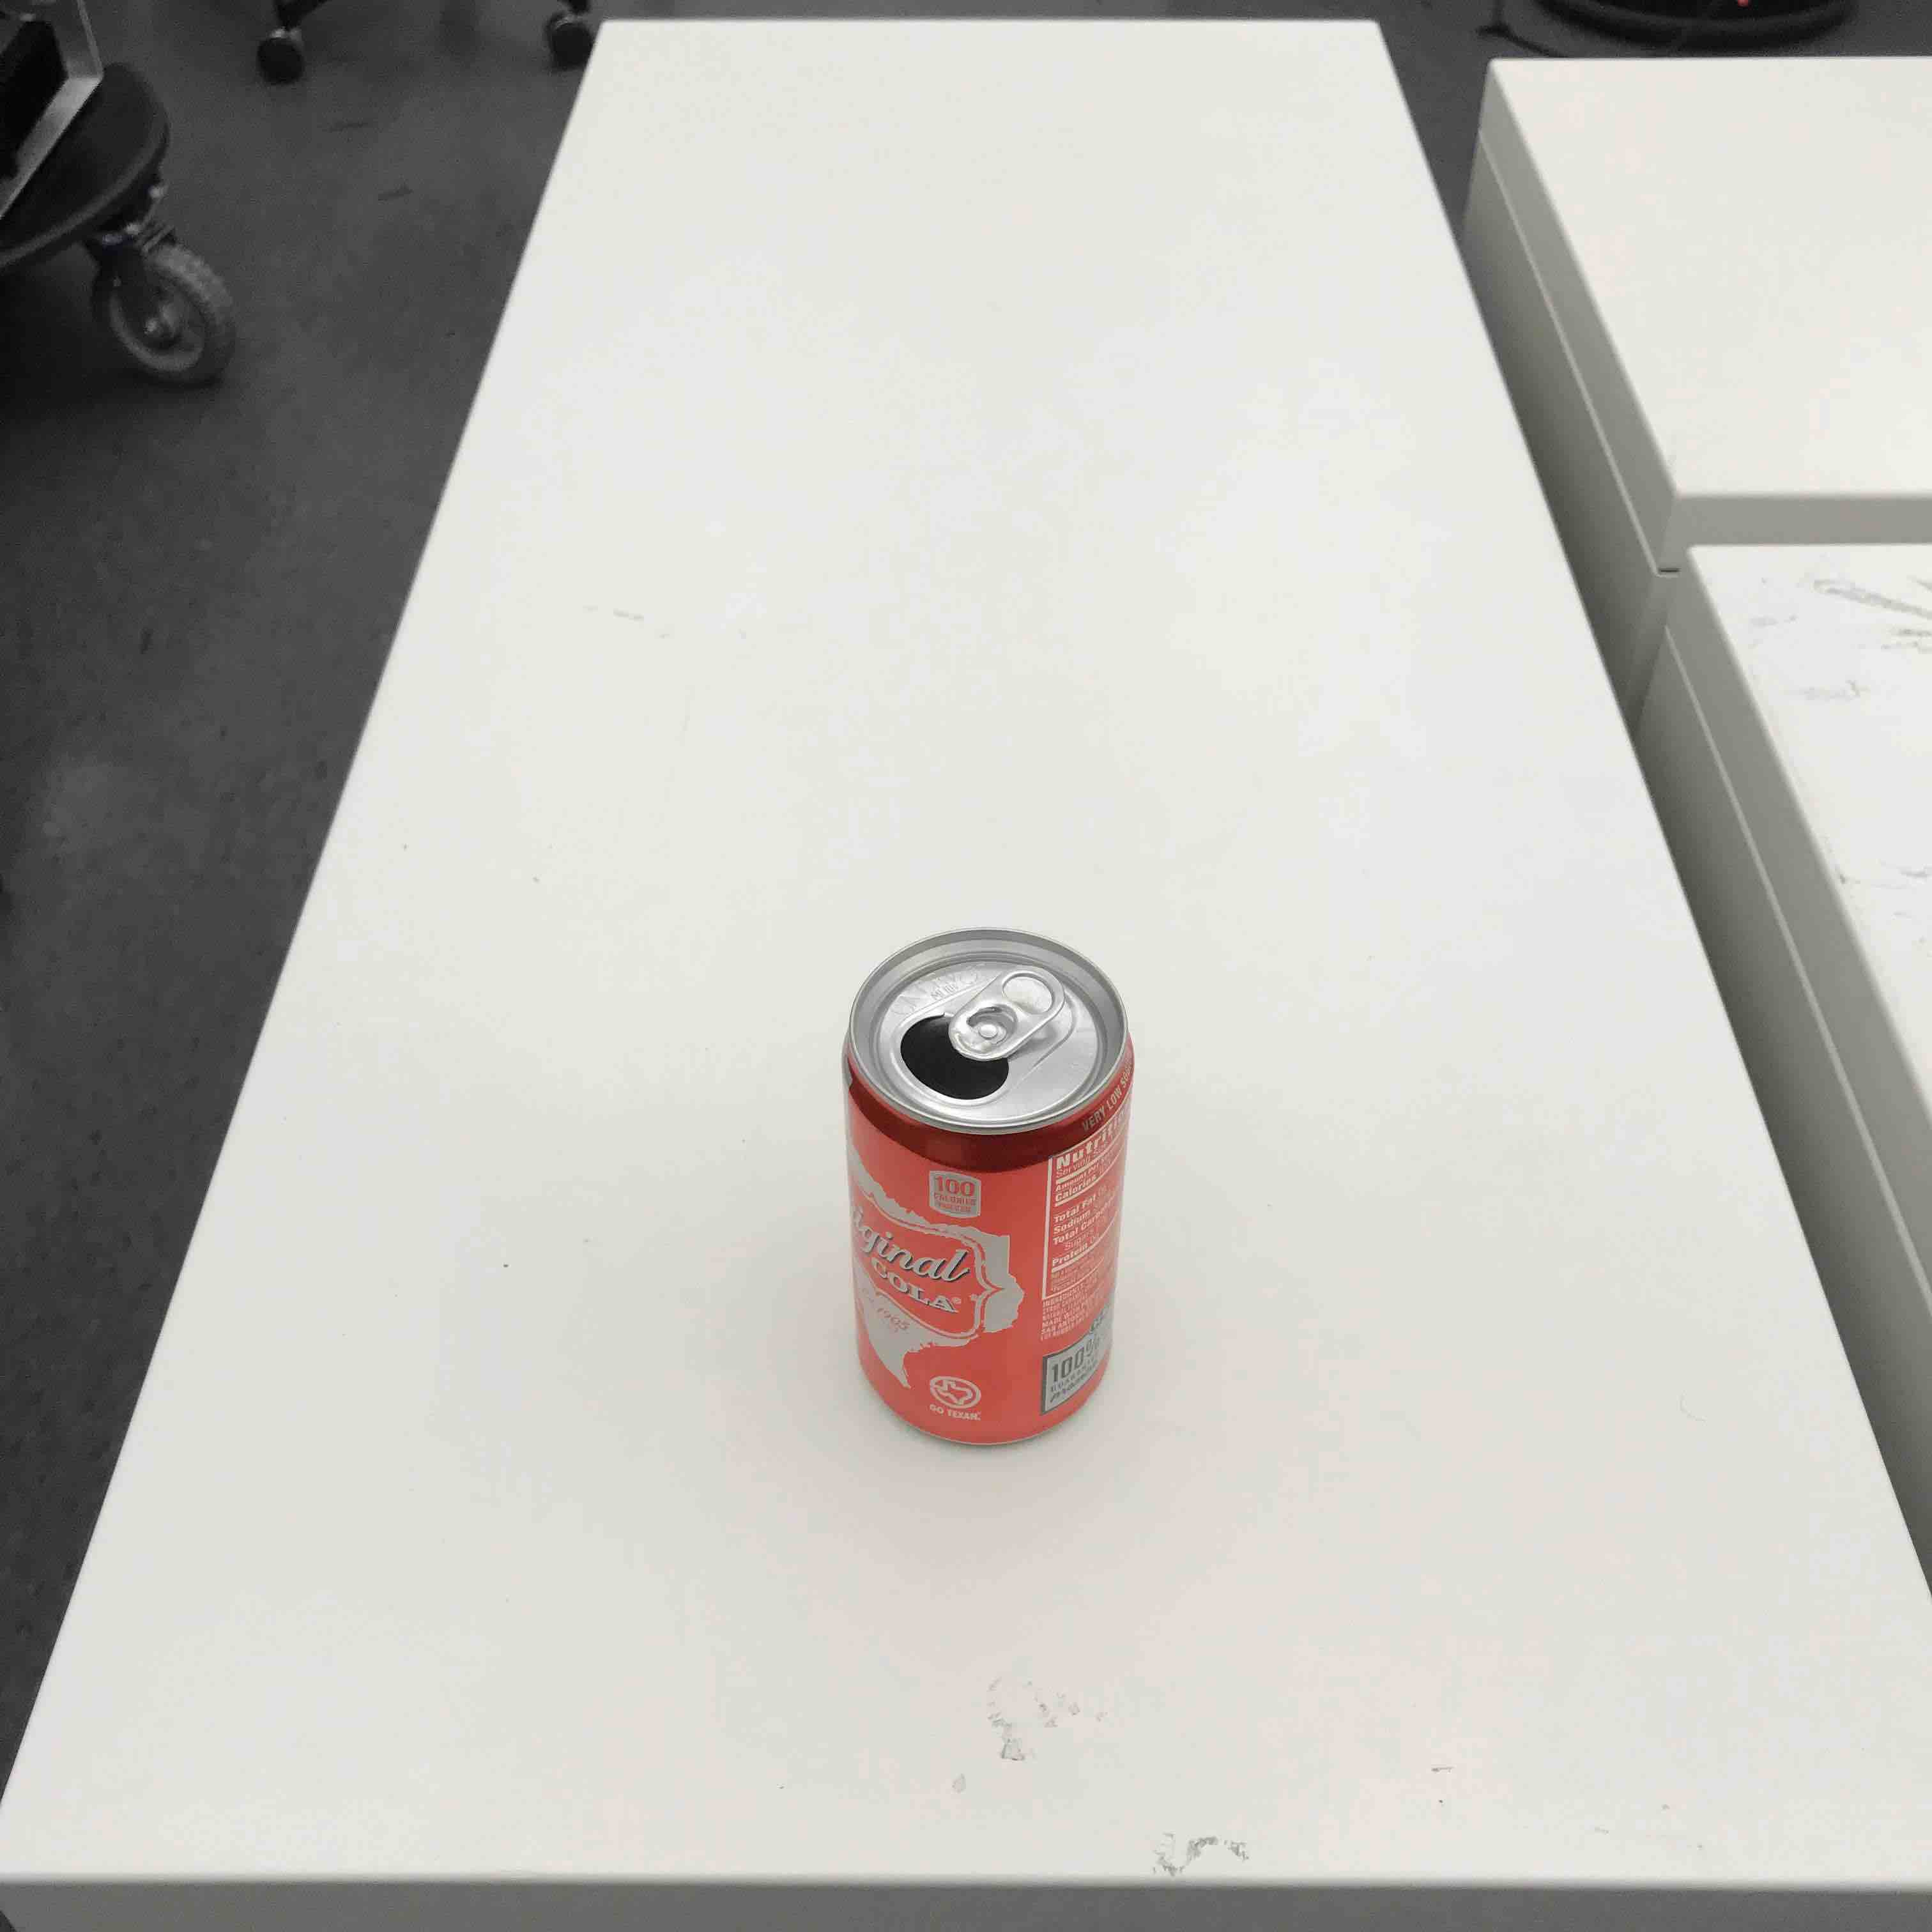
\includegraphics[width=0.3\linewidth]{figures/oidx_26.jpg} &
  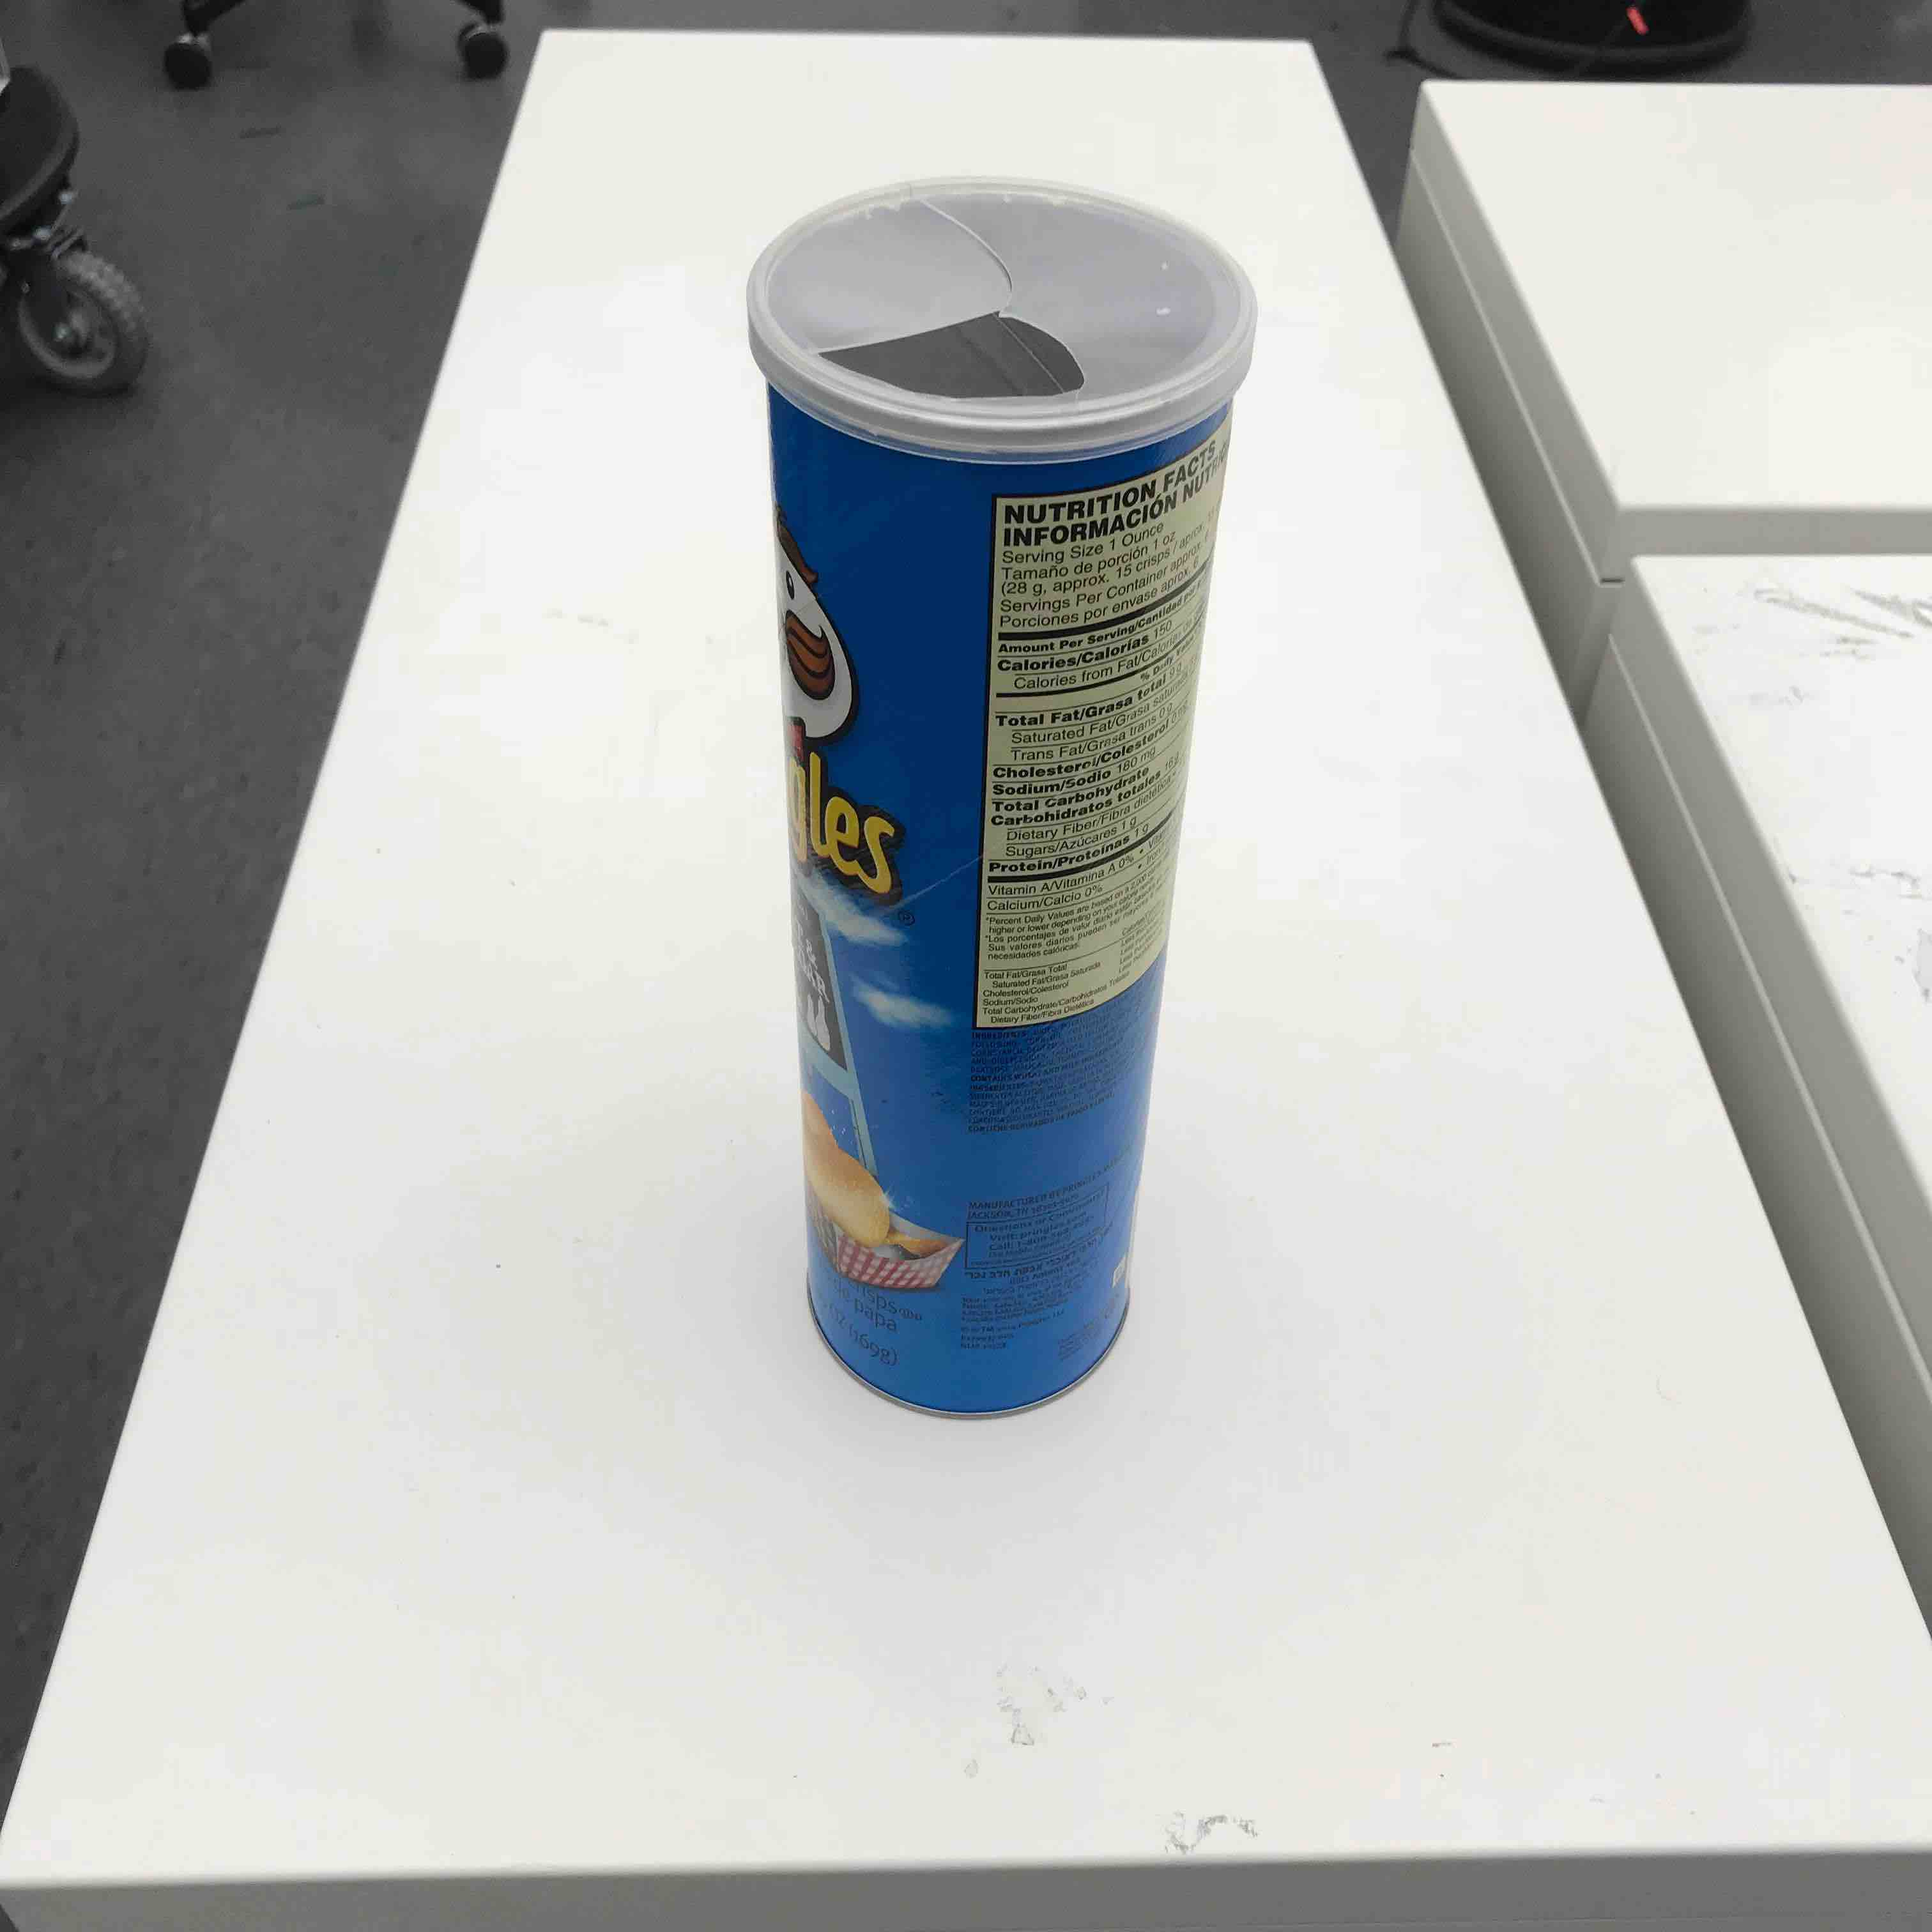
\includegraphics[width=0.3\linewidth]{figures/oidx_13.jpg} &
  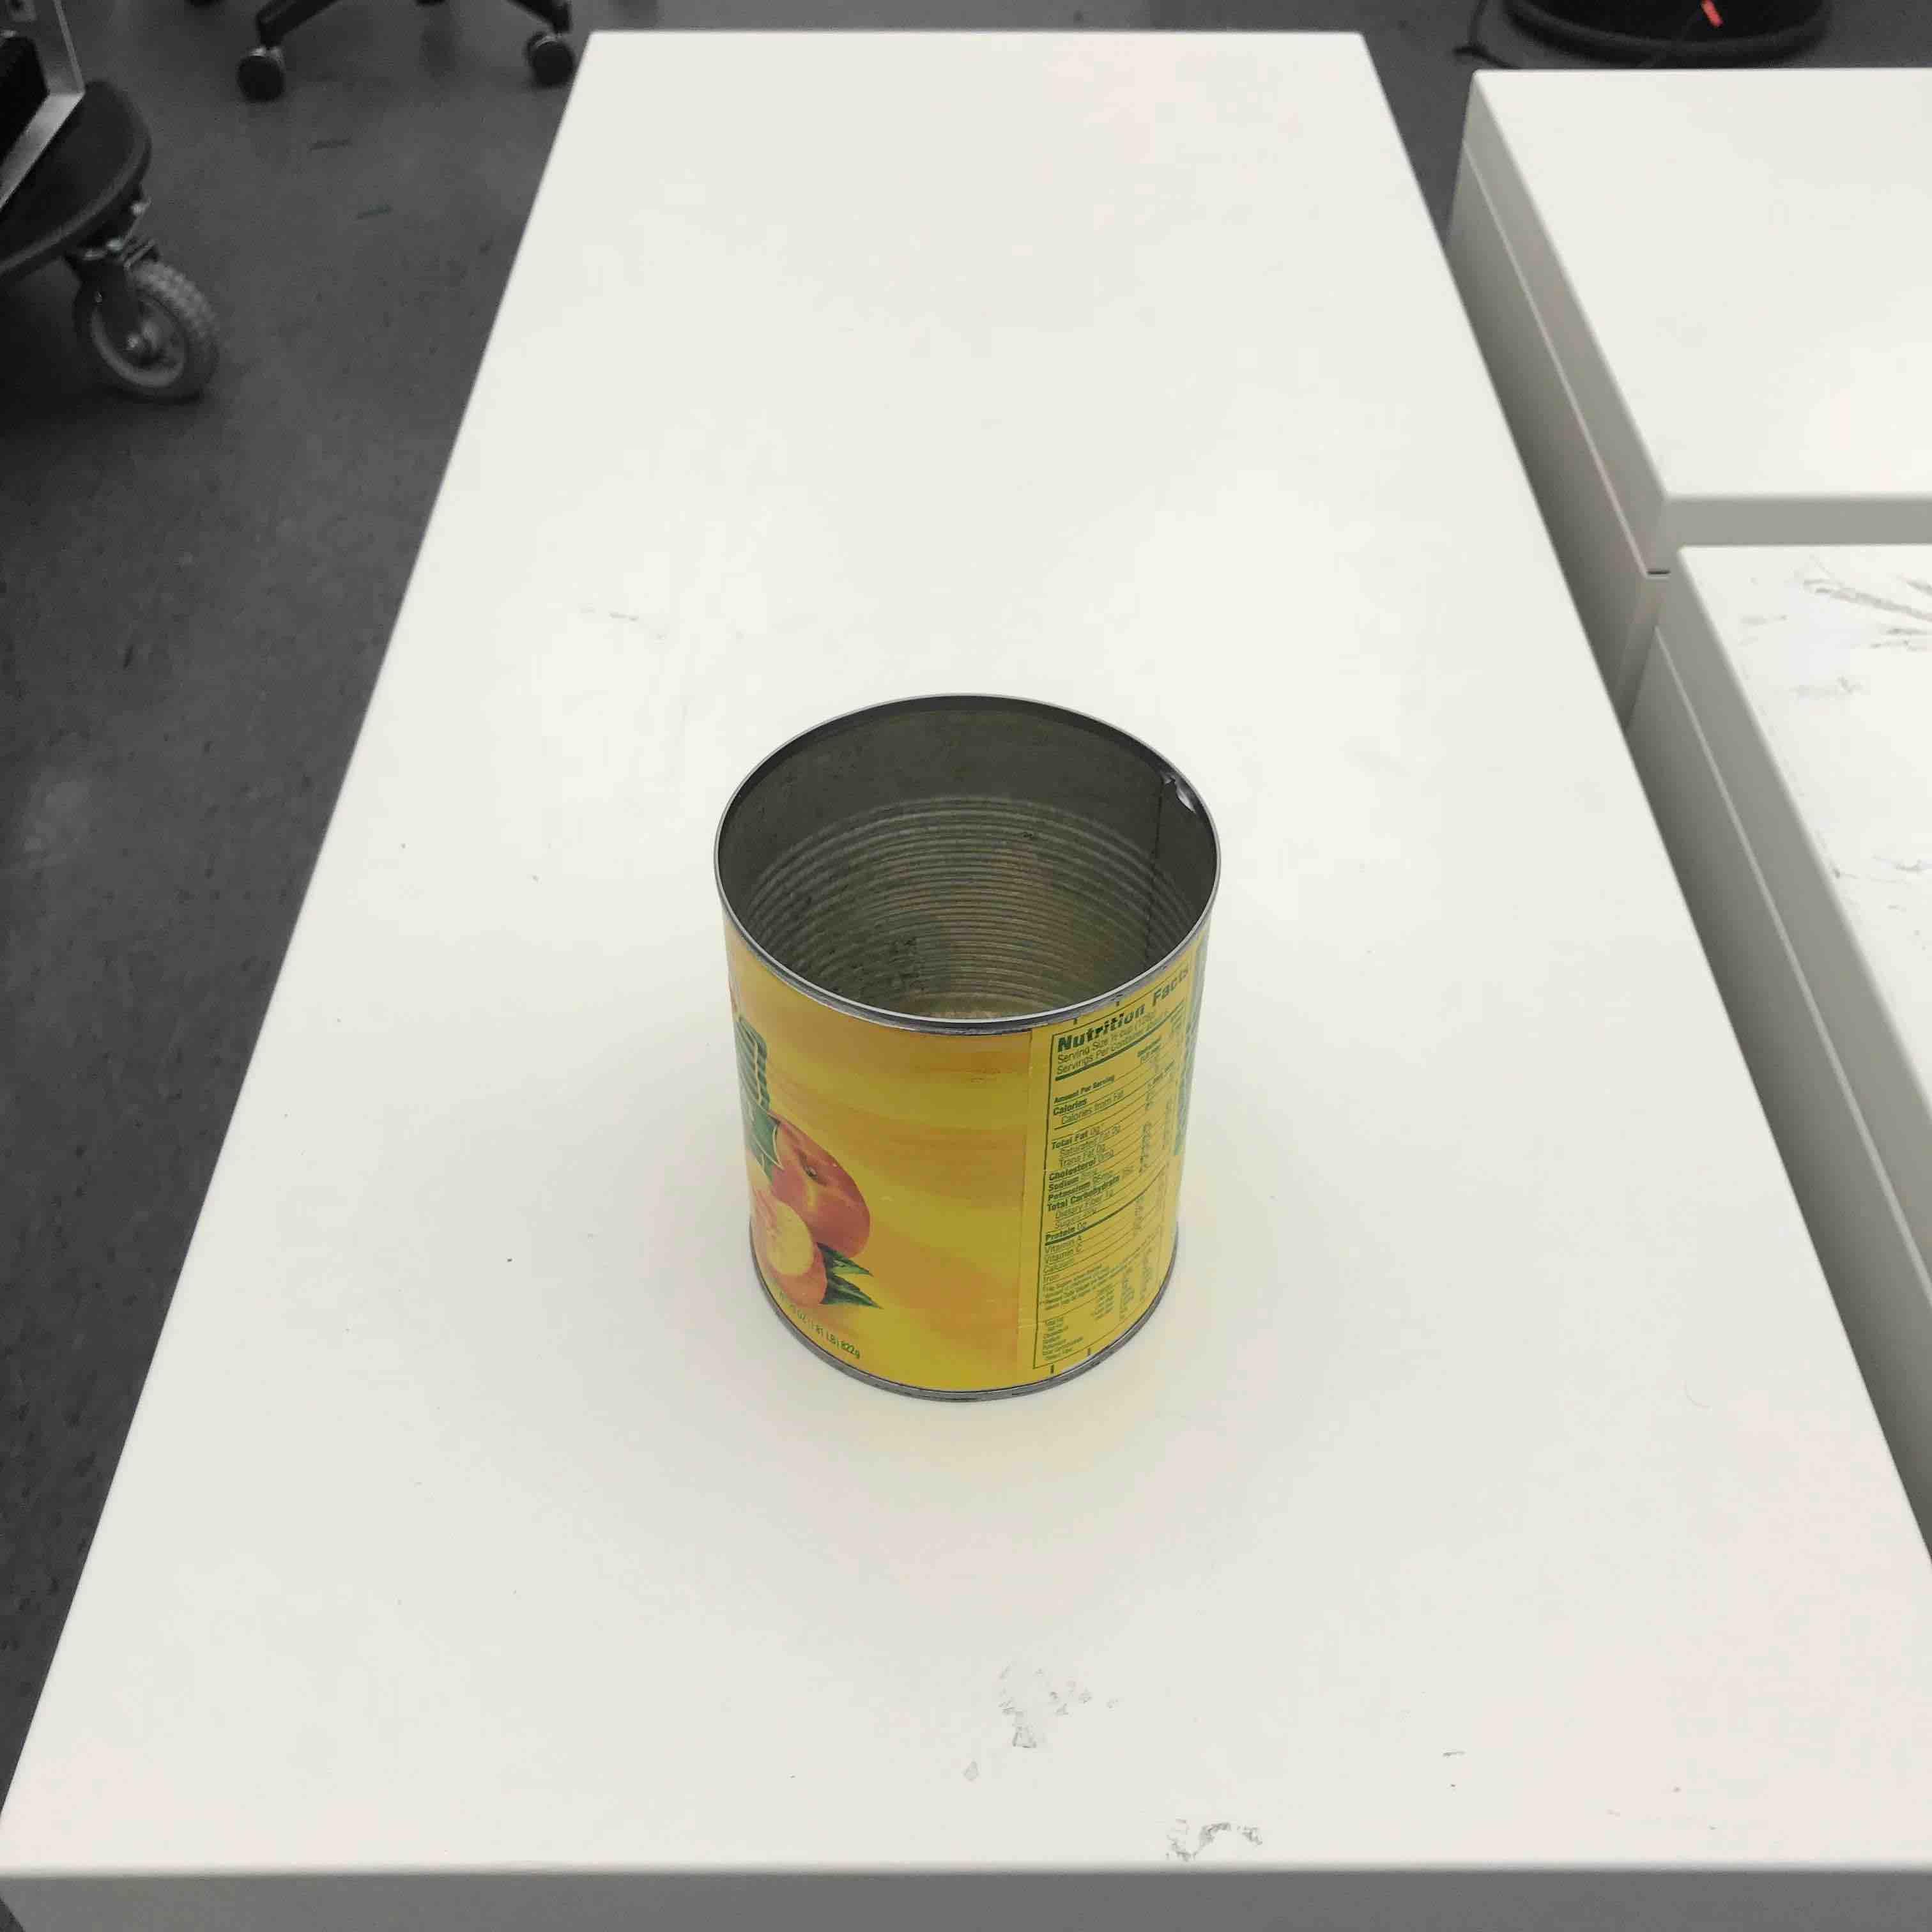
\includegraphics[width=0.3\linewidth]{figures/oidx_11.jpg} \\
  0.32 & 0.22 & 0.2 \\
  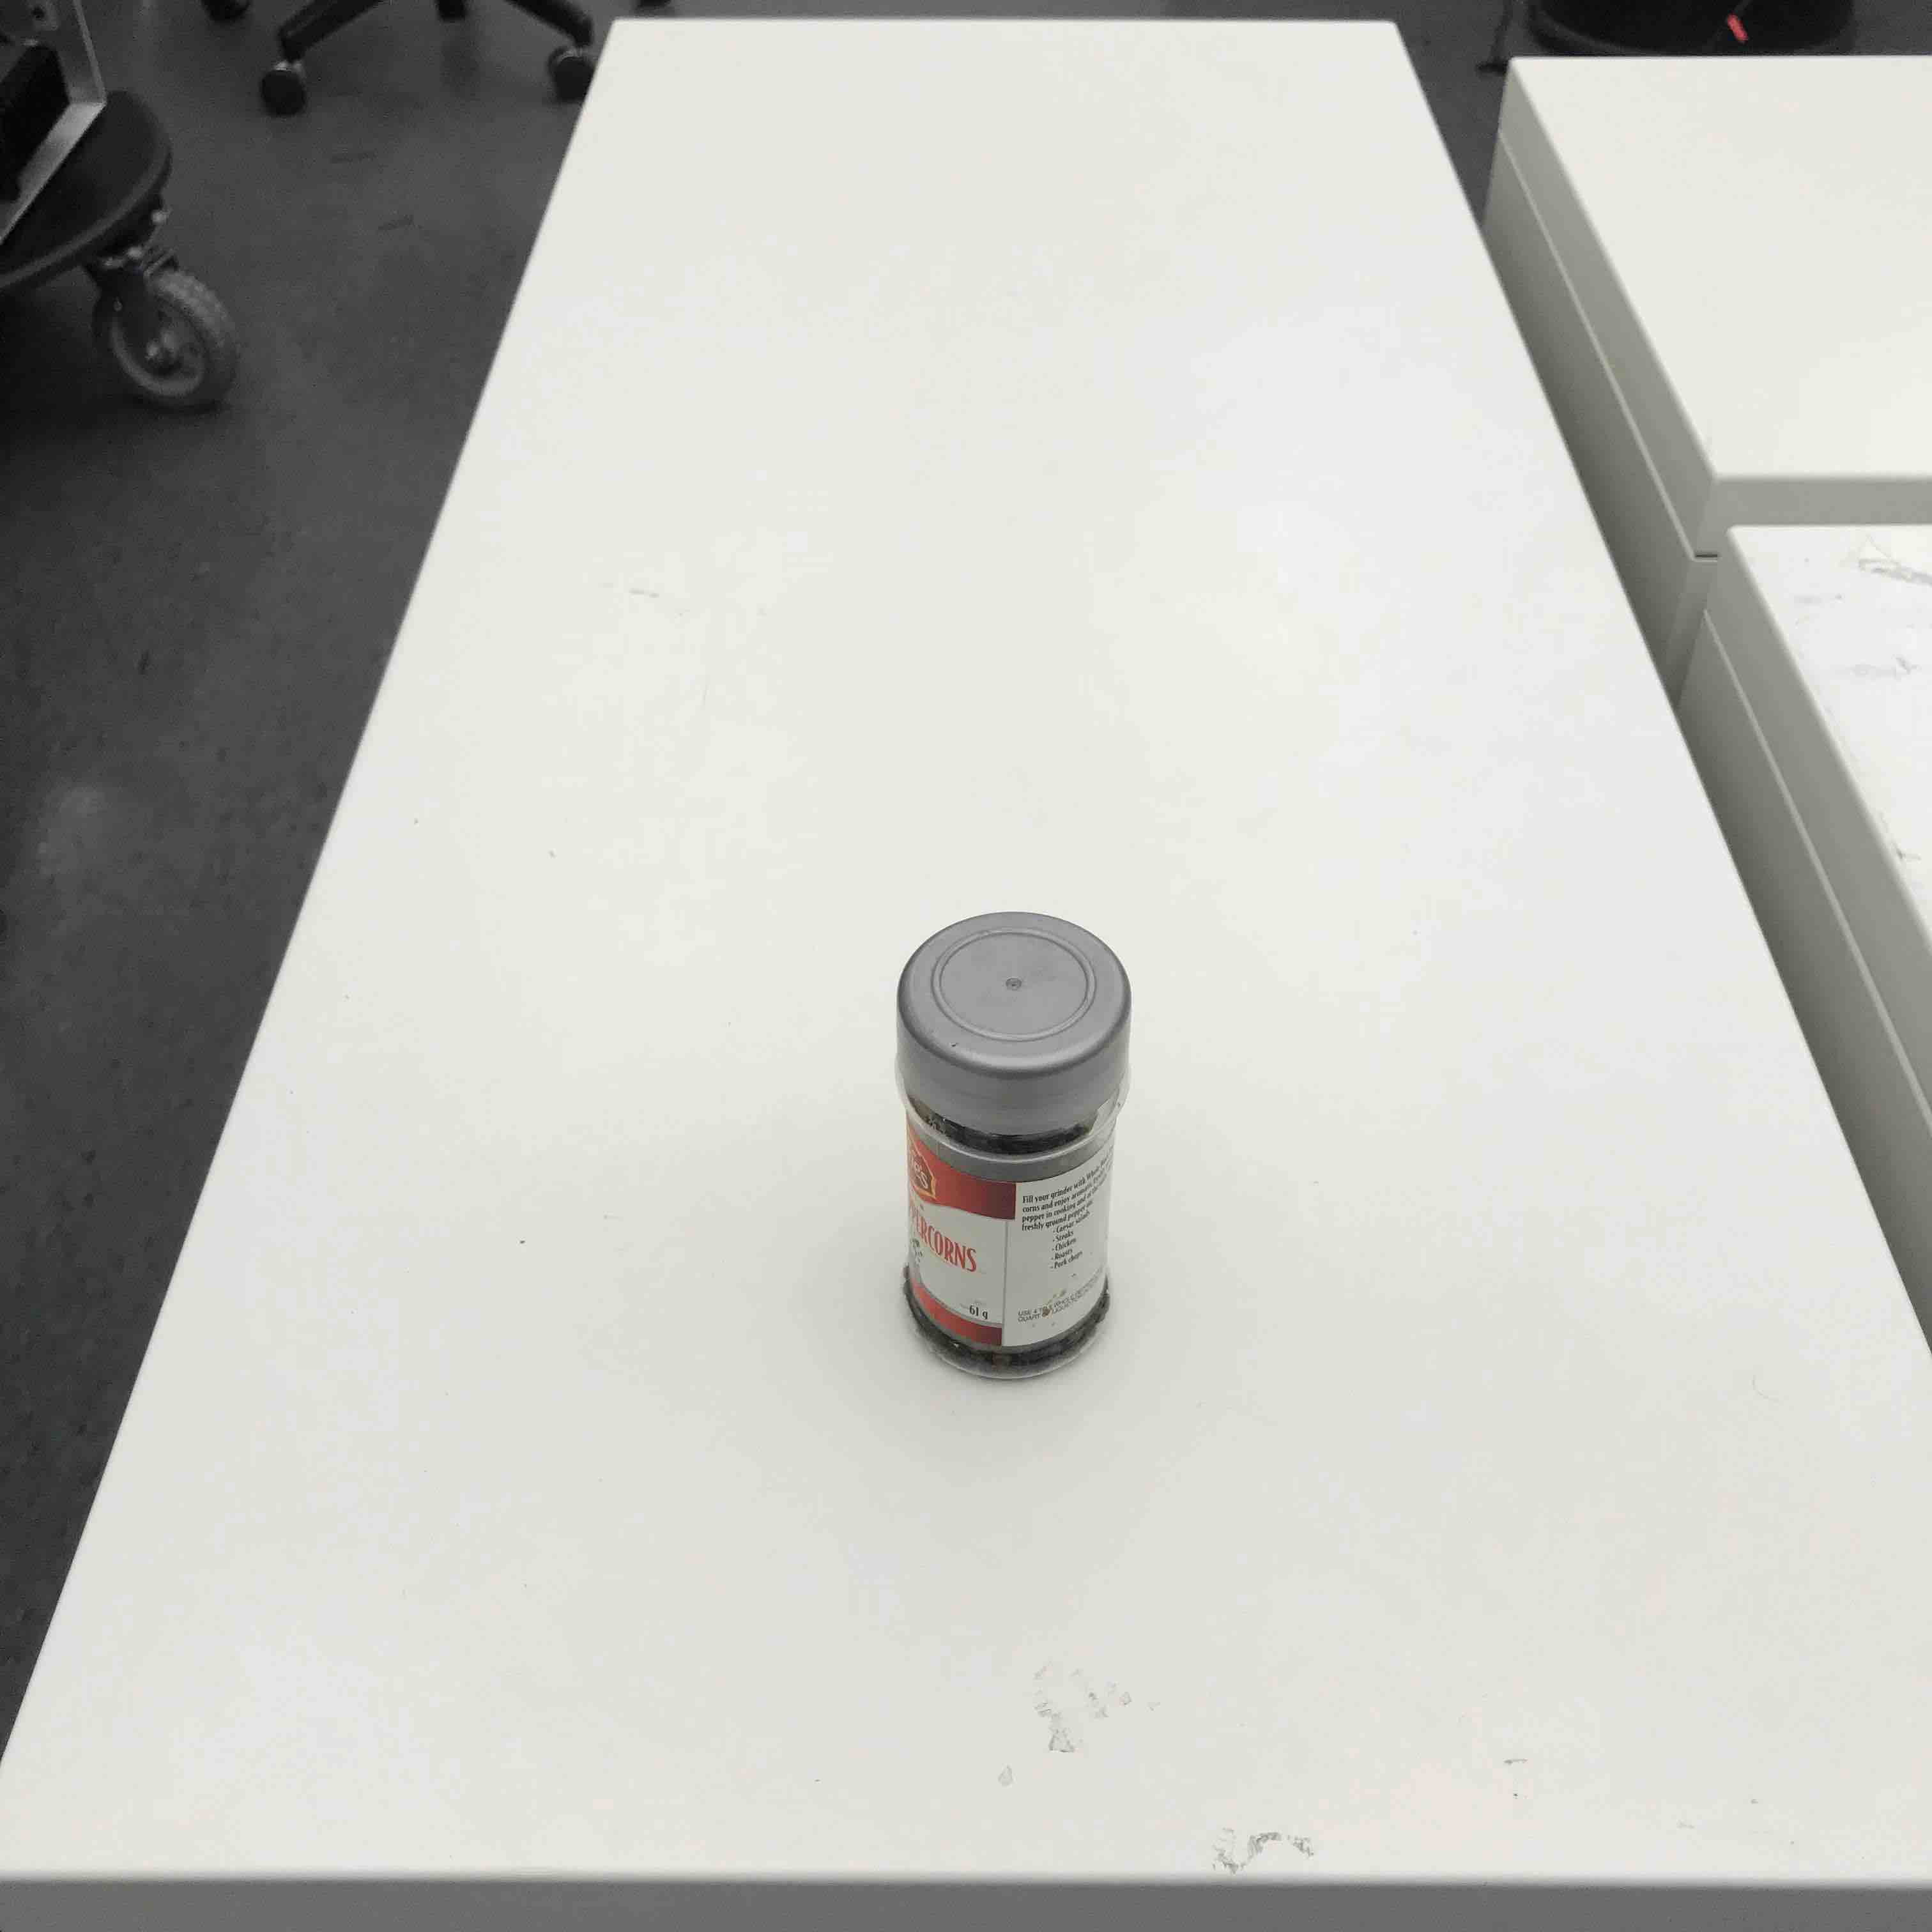
\includegraphics[width=0.3\linewidth]{figures/oidx_25.jpg} &
  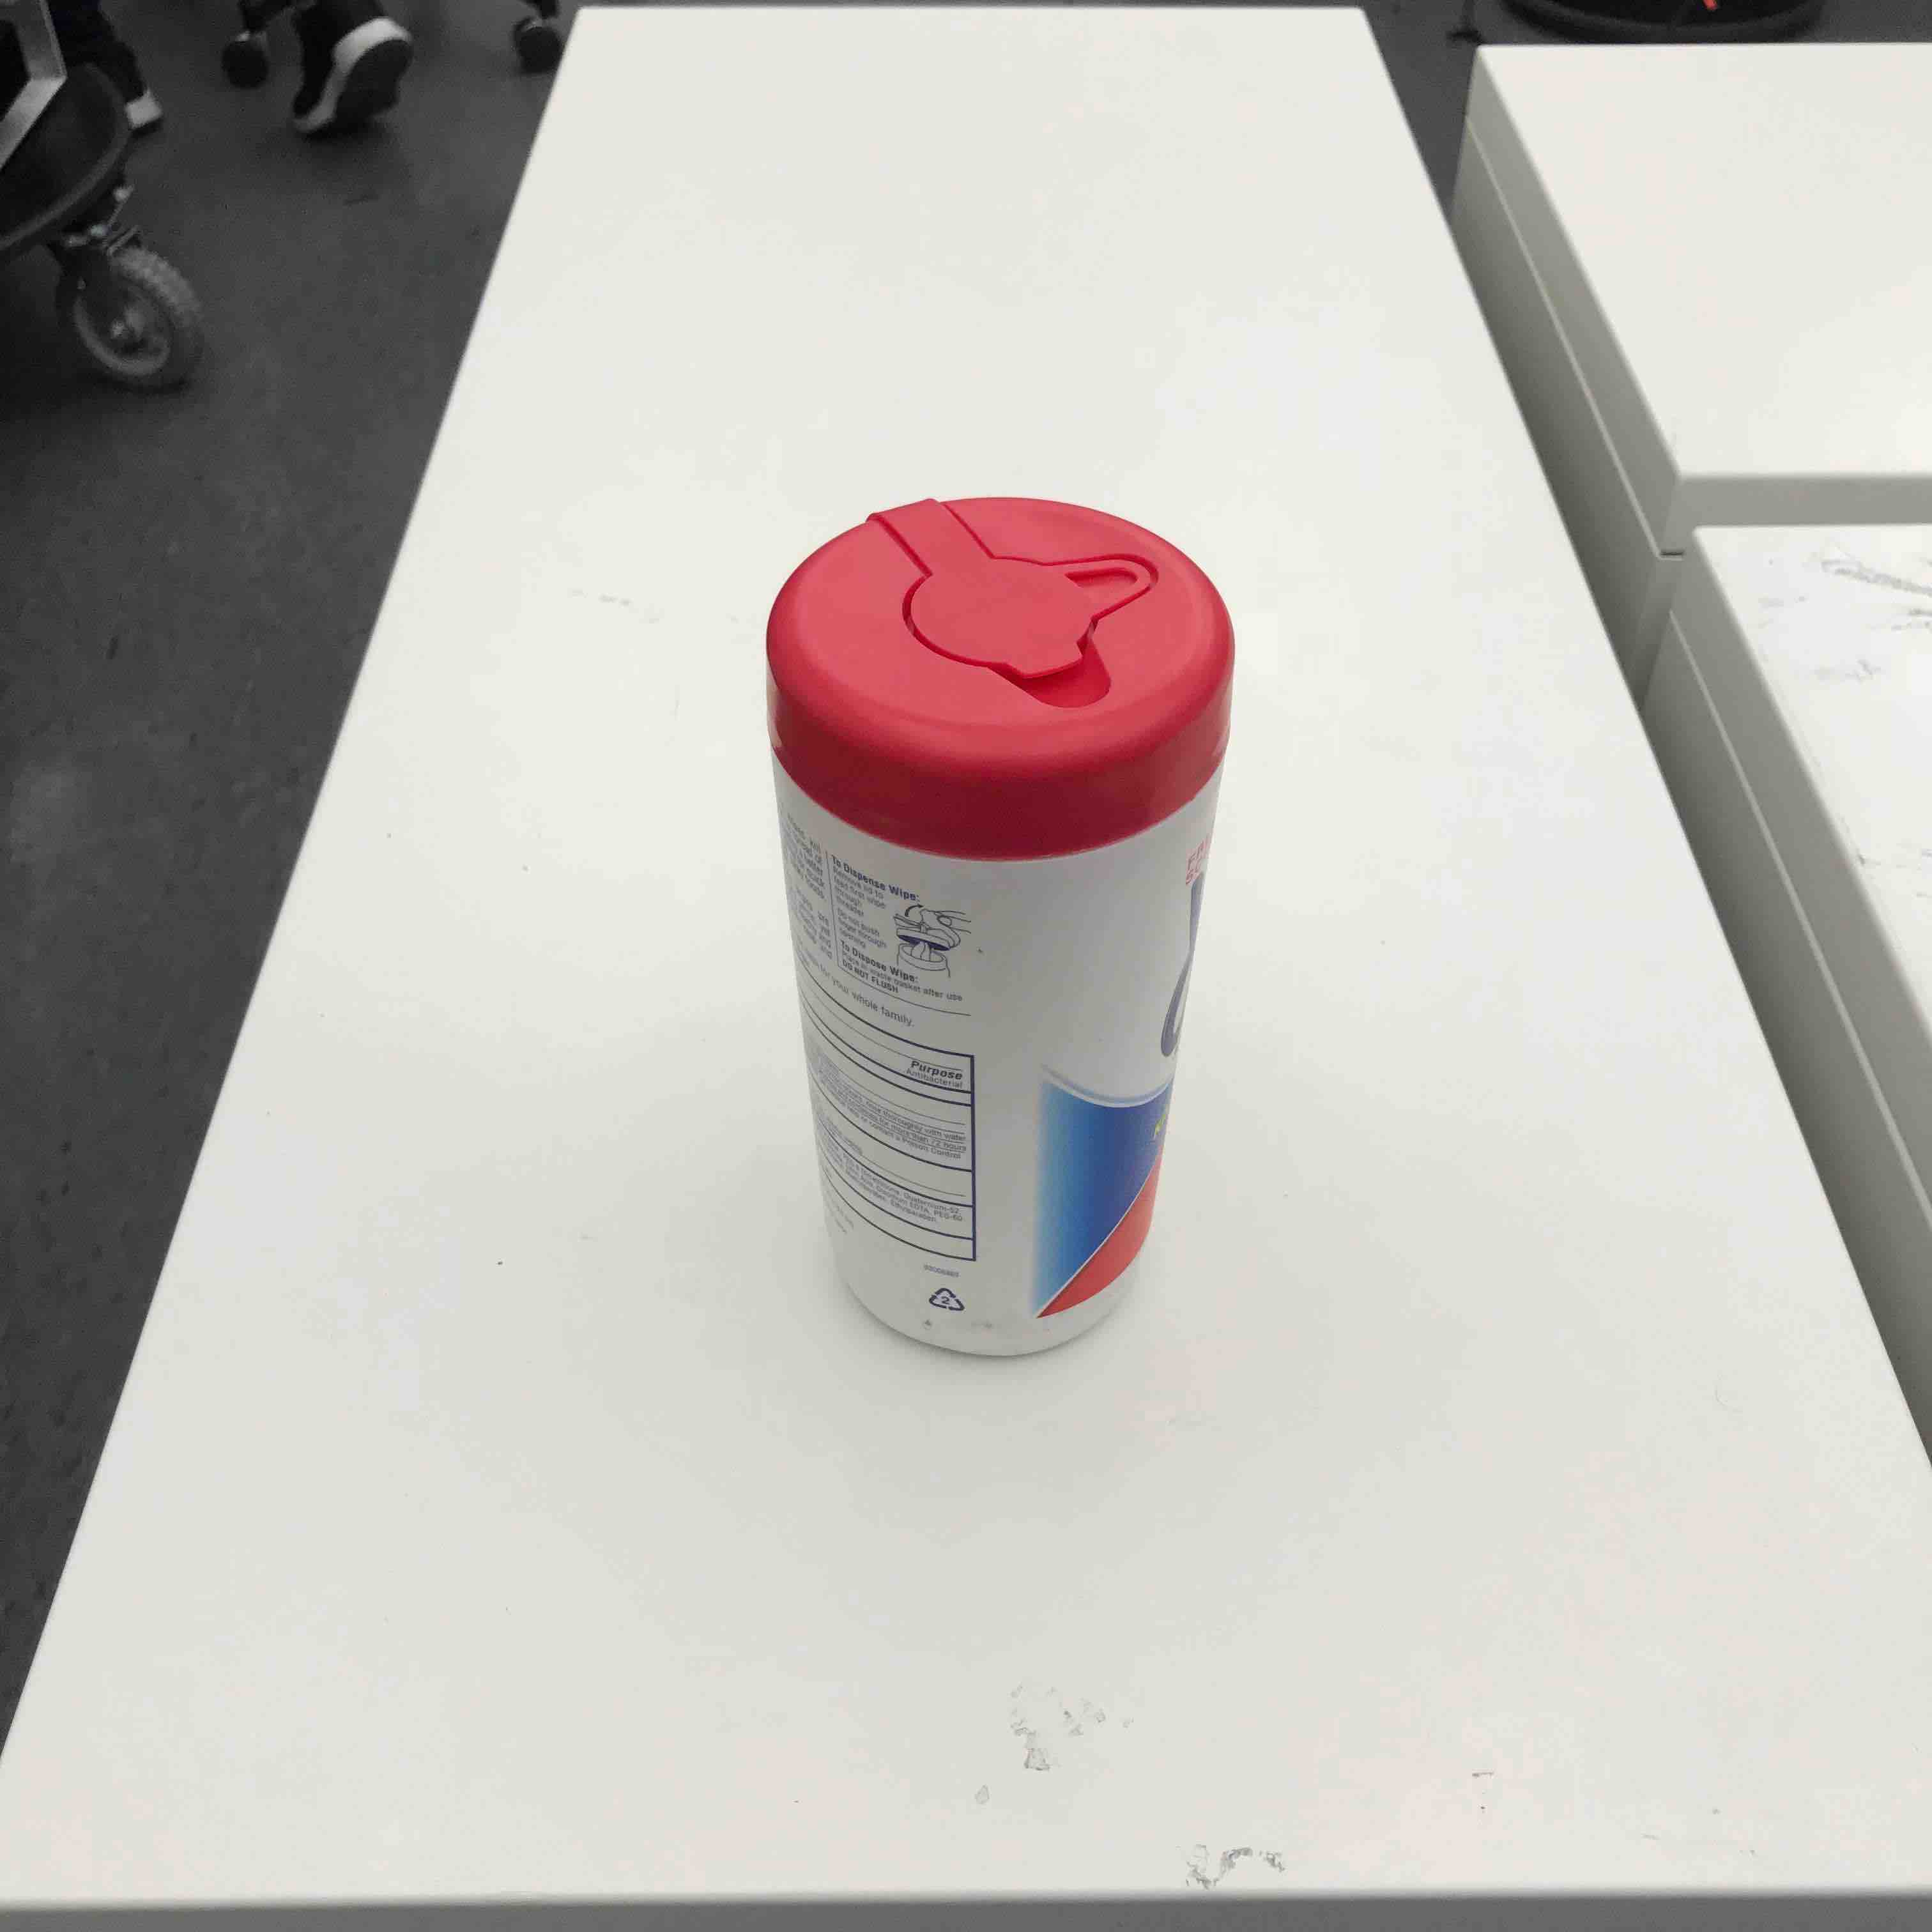
\includegraphics[width=0.3\linewidth]{figures/oidx_12.jpg} &
  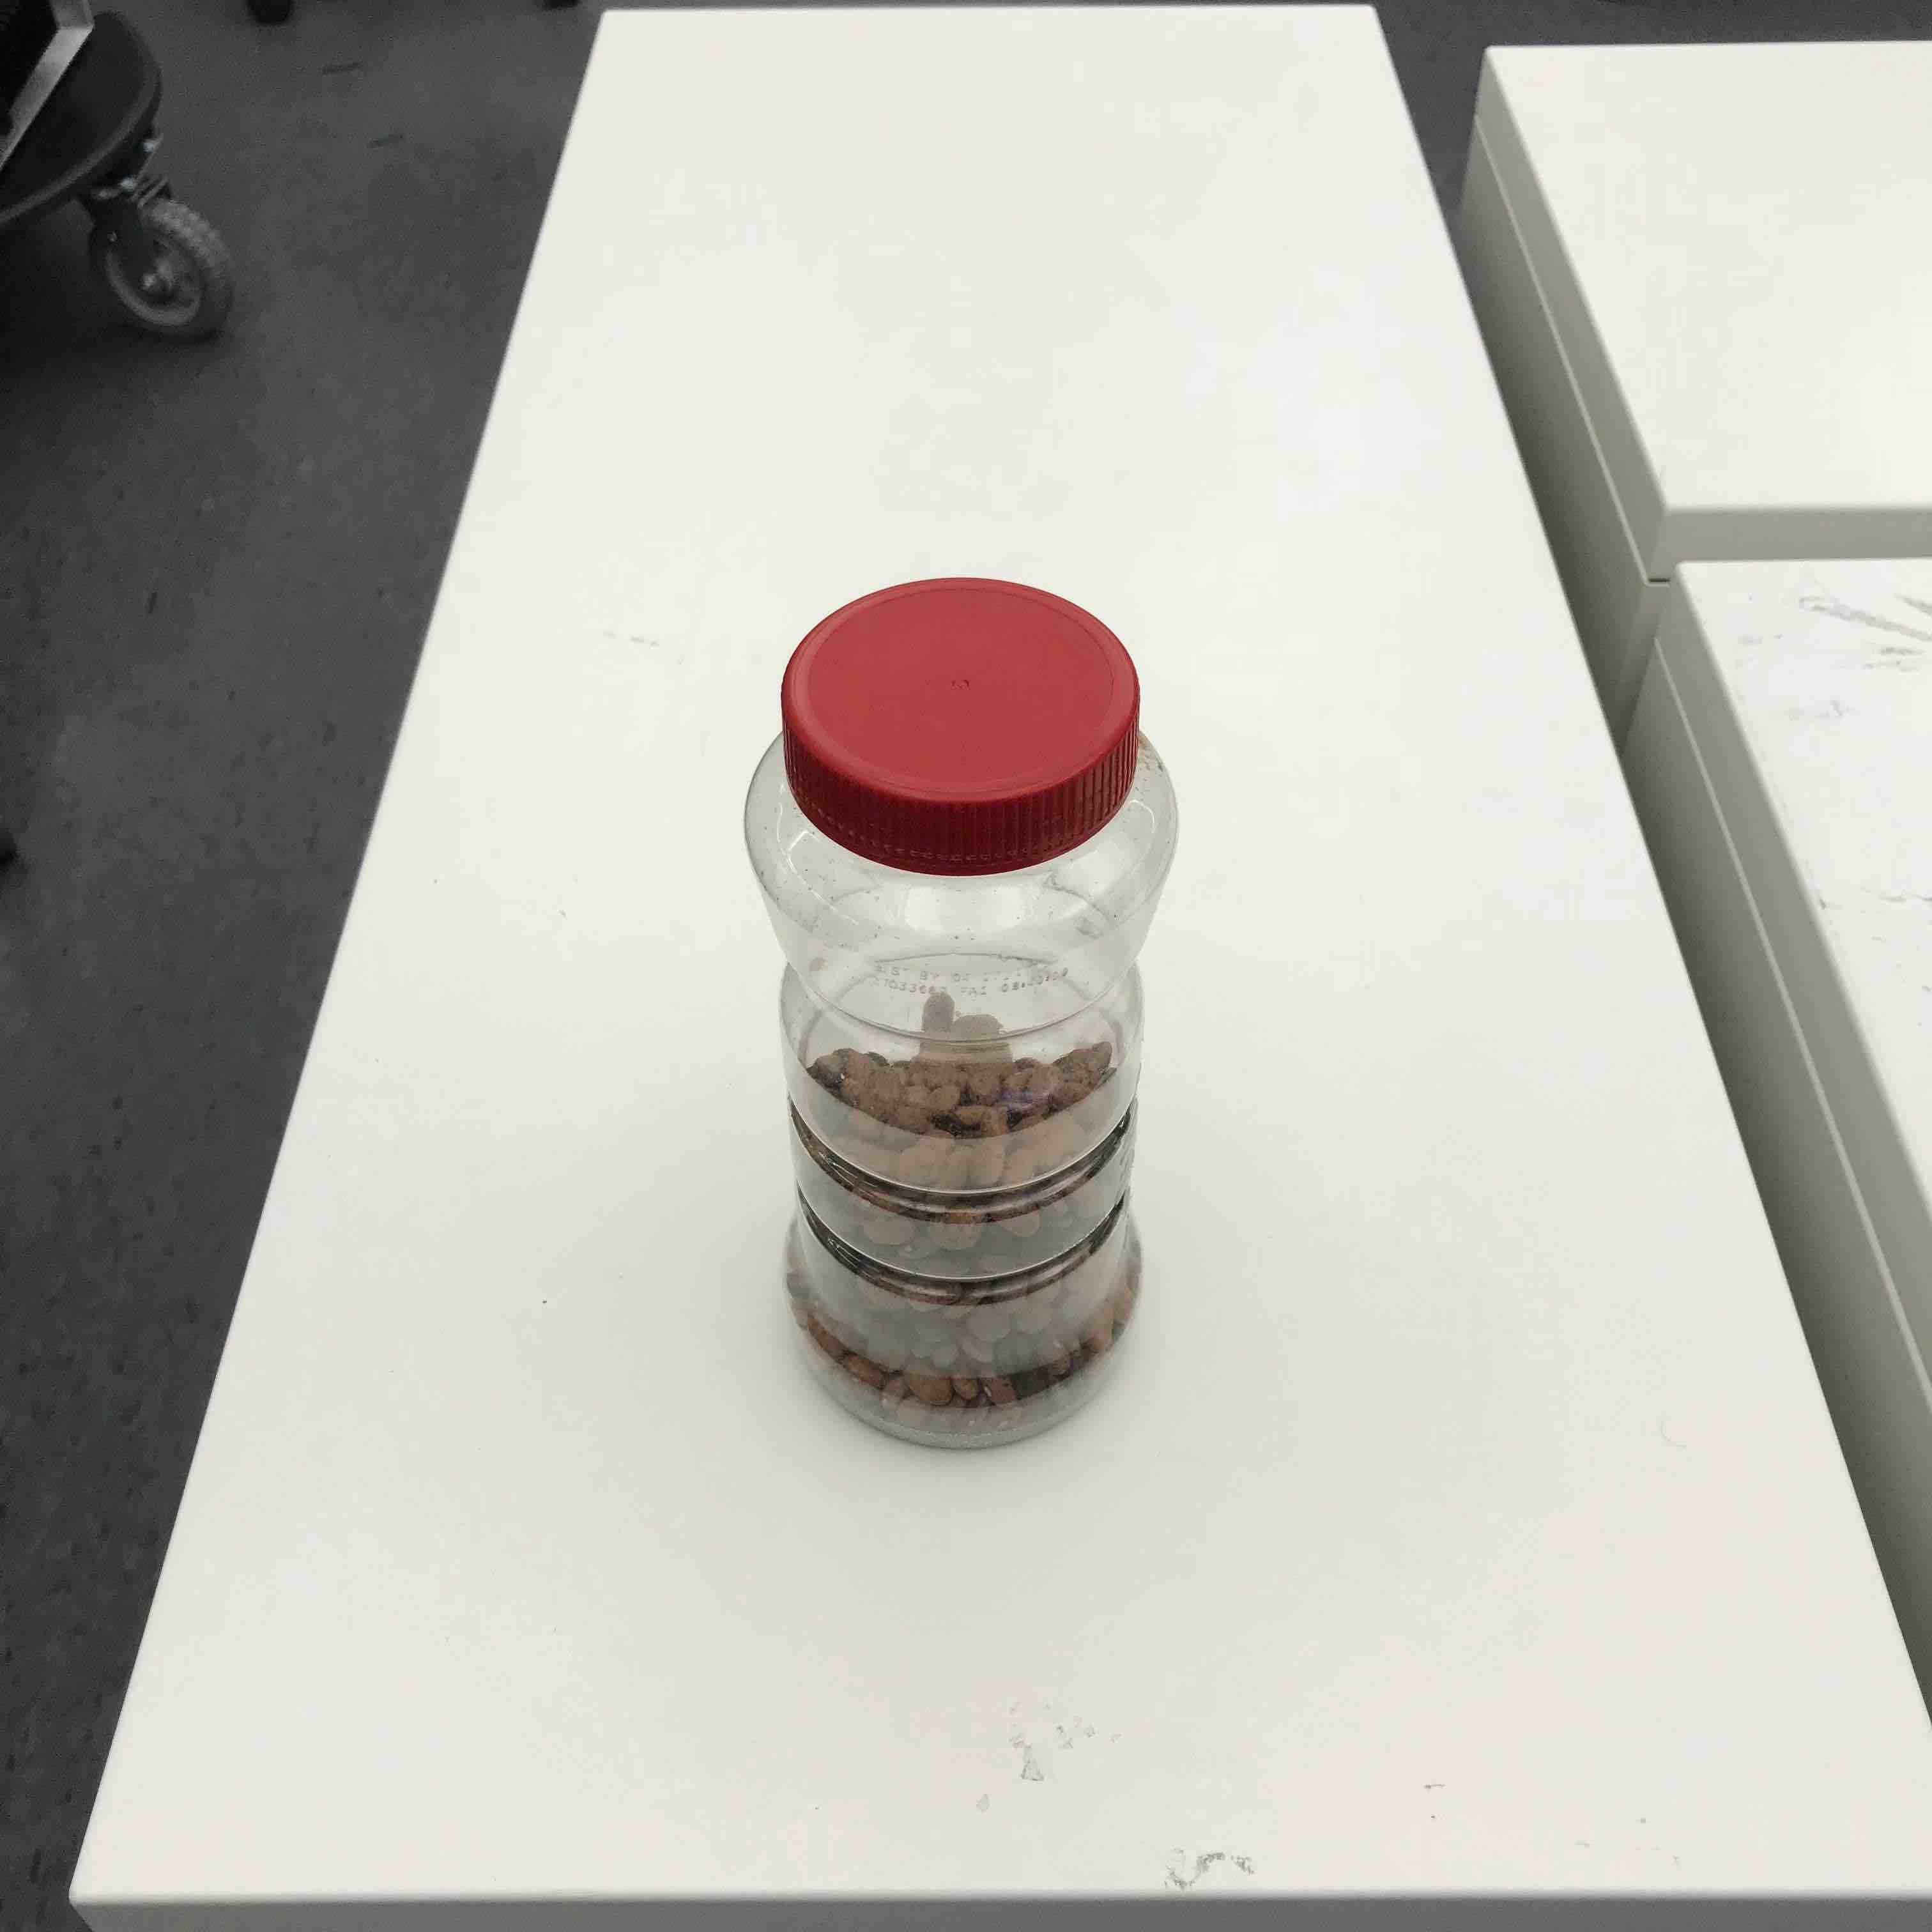
\includegraphics[width=0.3\linewidth]{figures/oidx_22.jpg} \\
  0.13 & 0.07 & 0.03 \\
  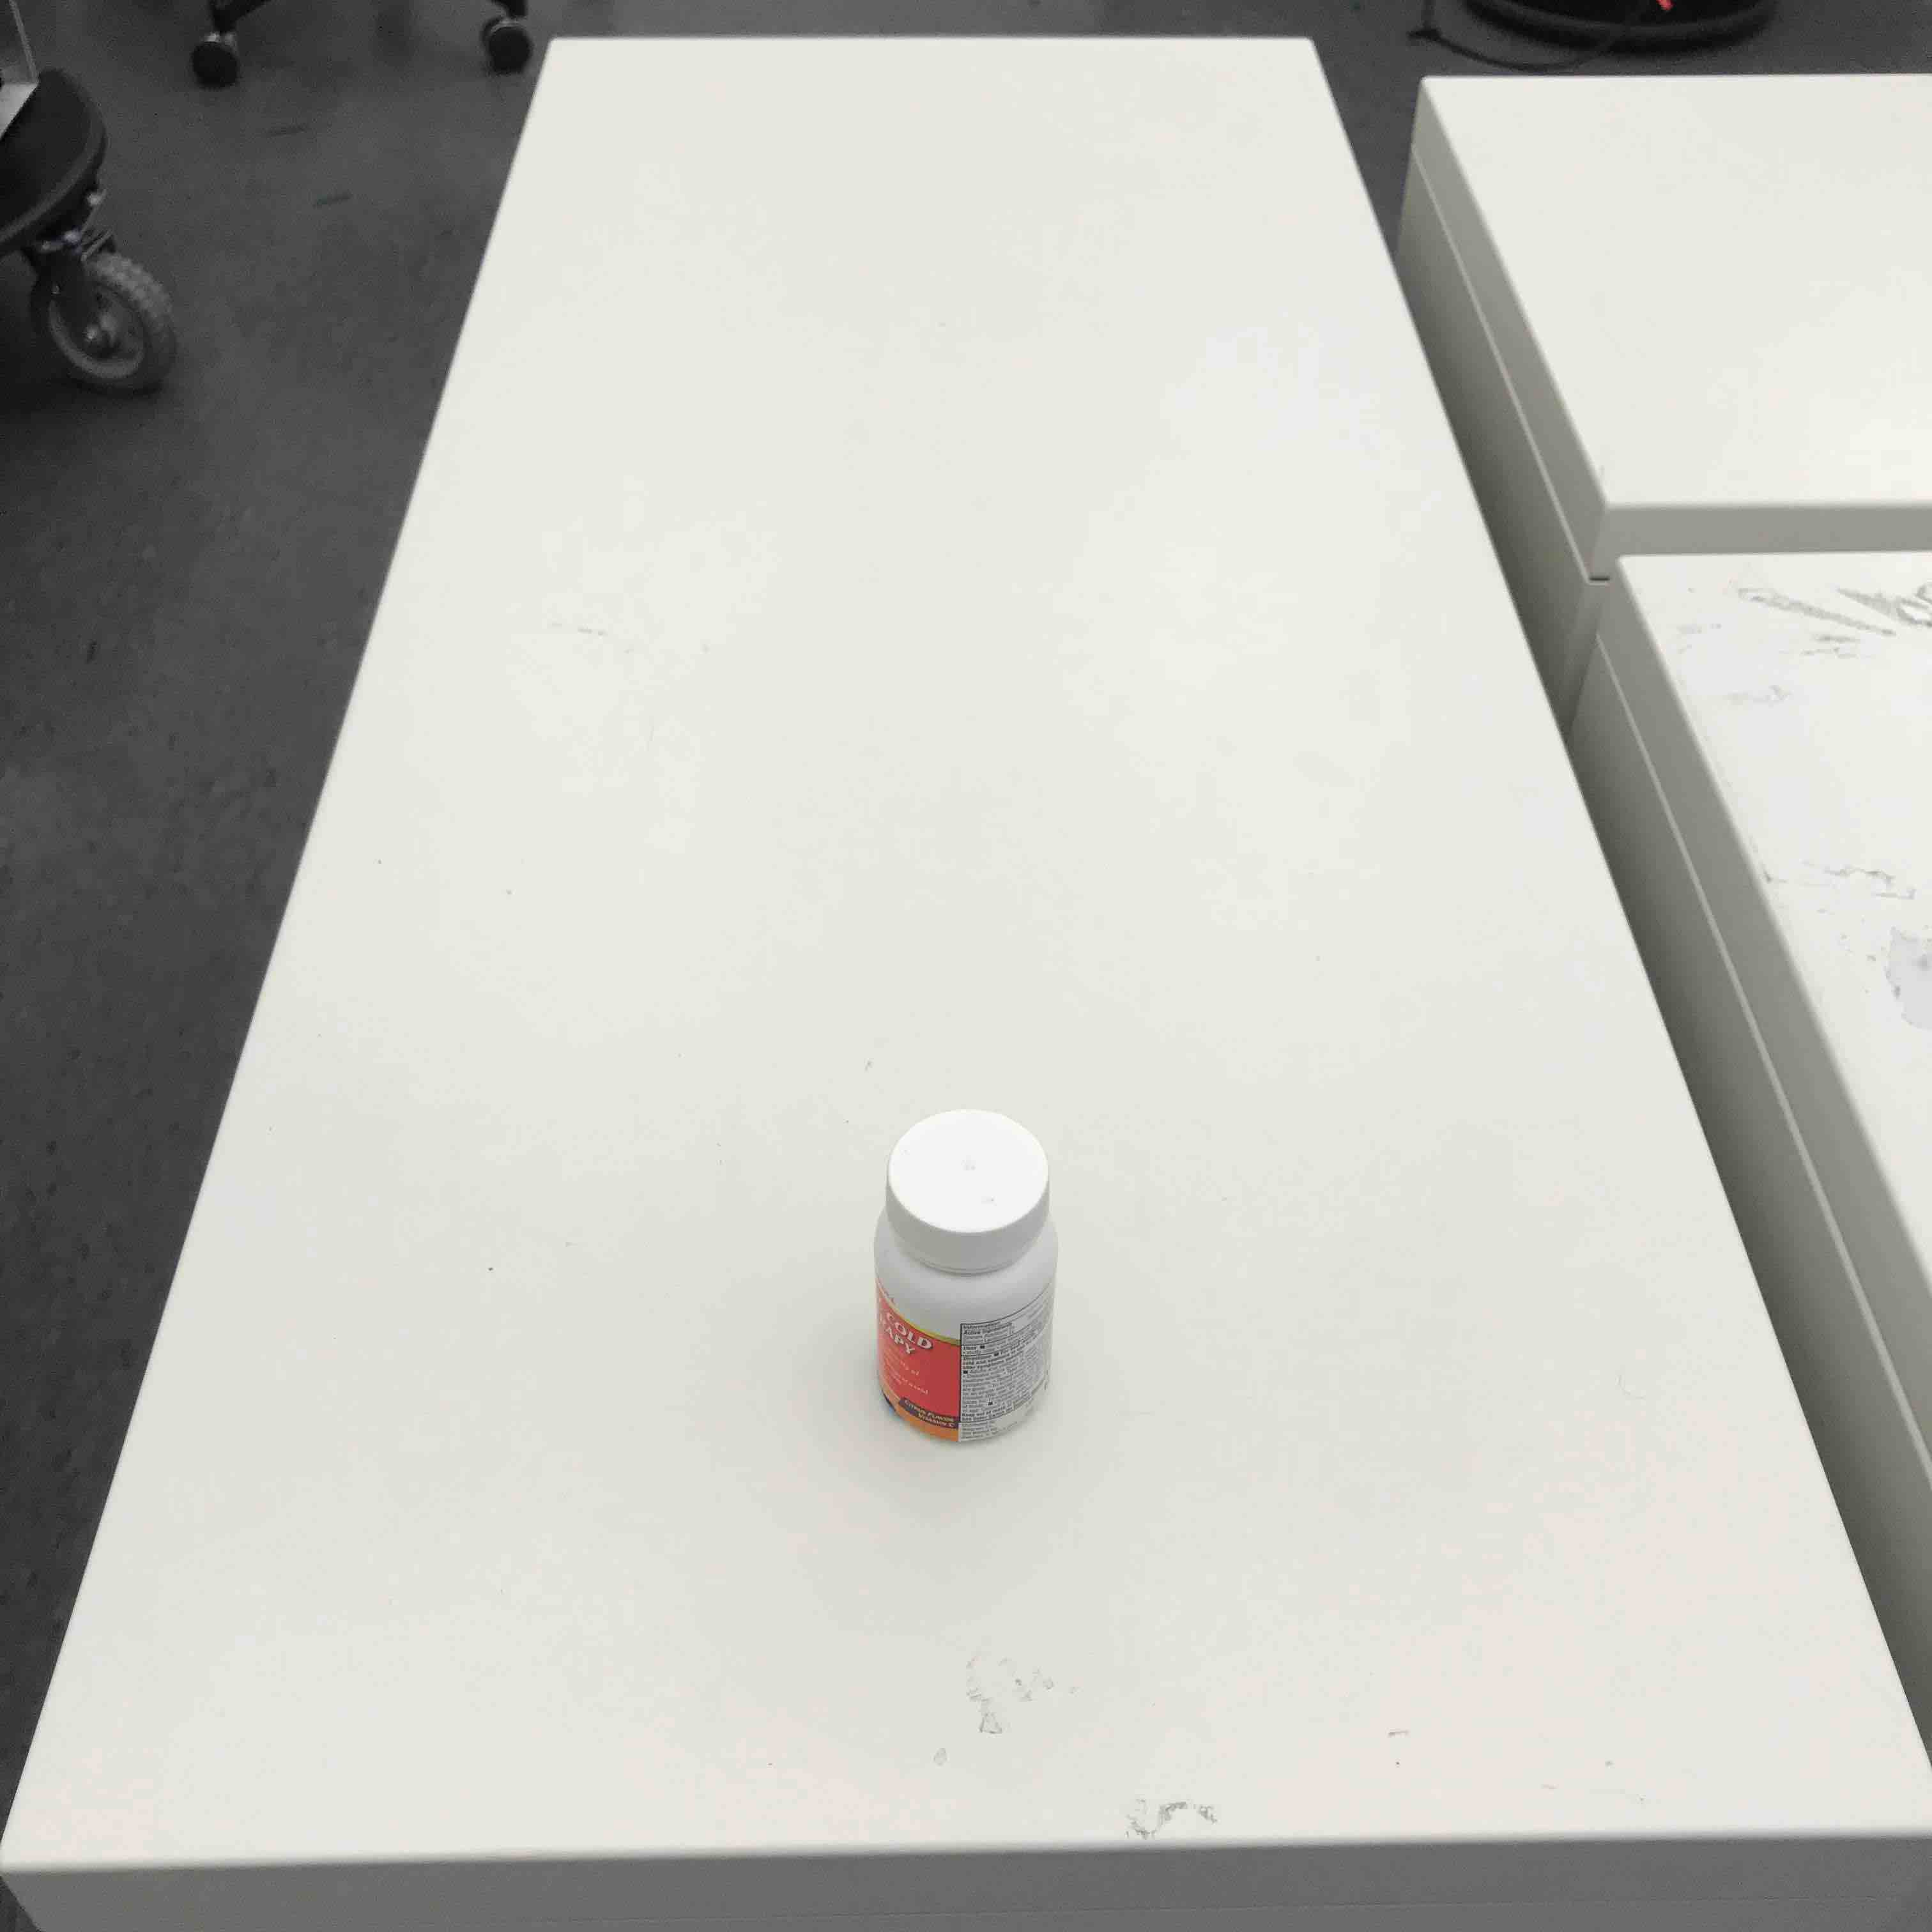
\includegraphics[width=0.3\linewidth]{figures/oidx_6.jpg} &
  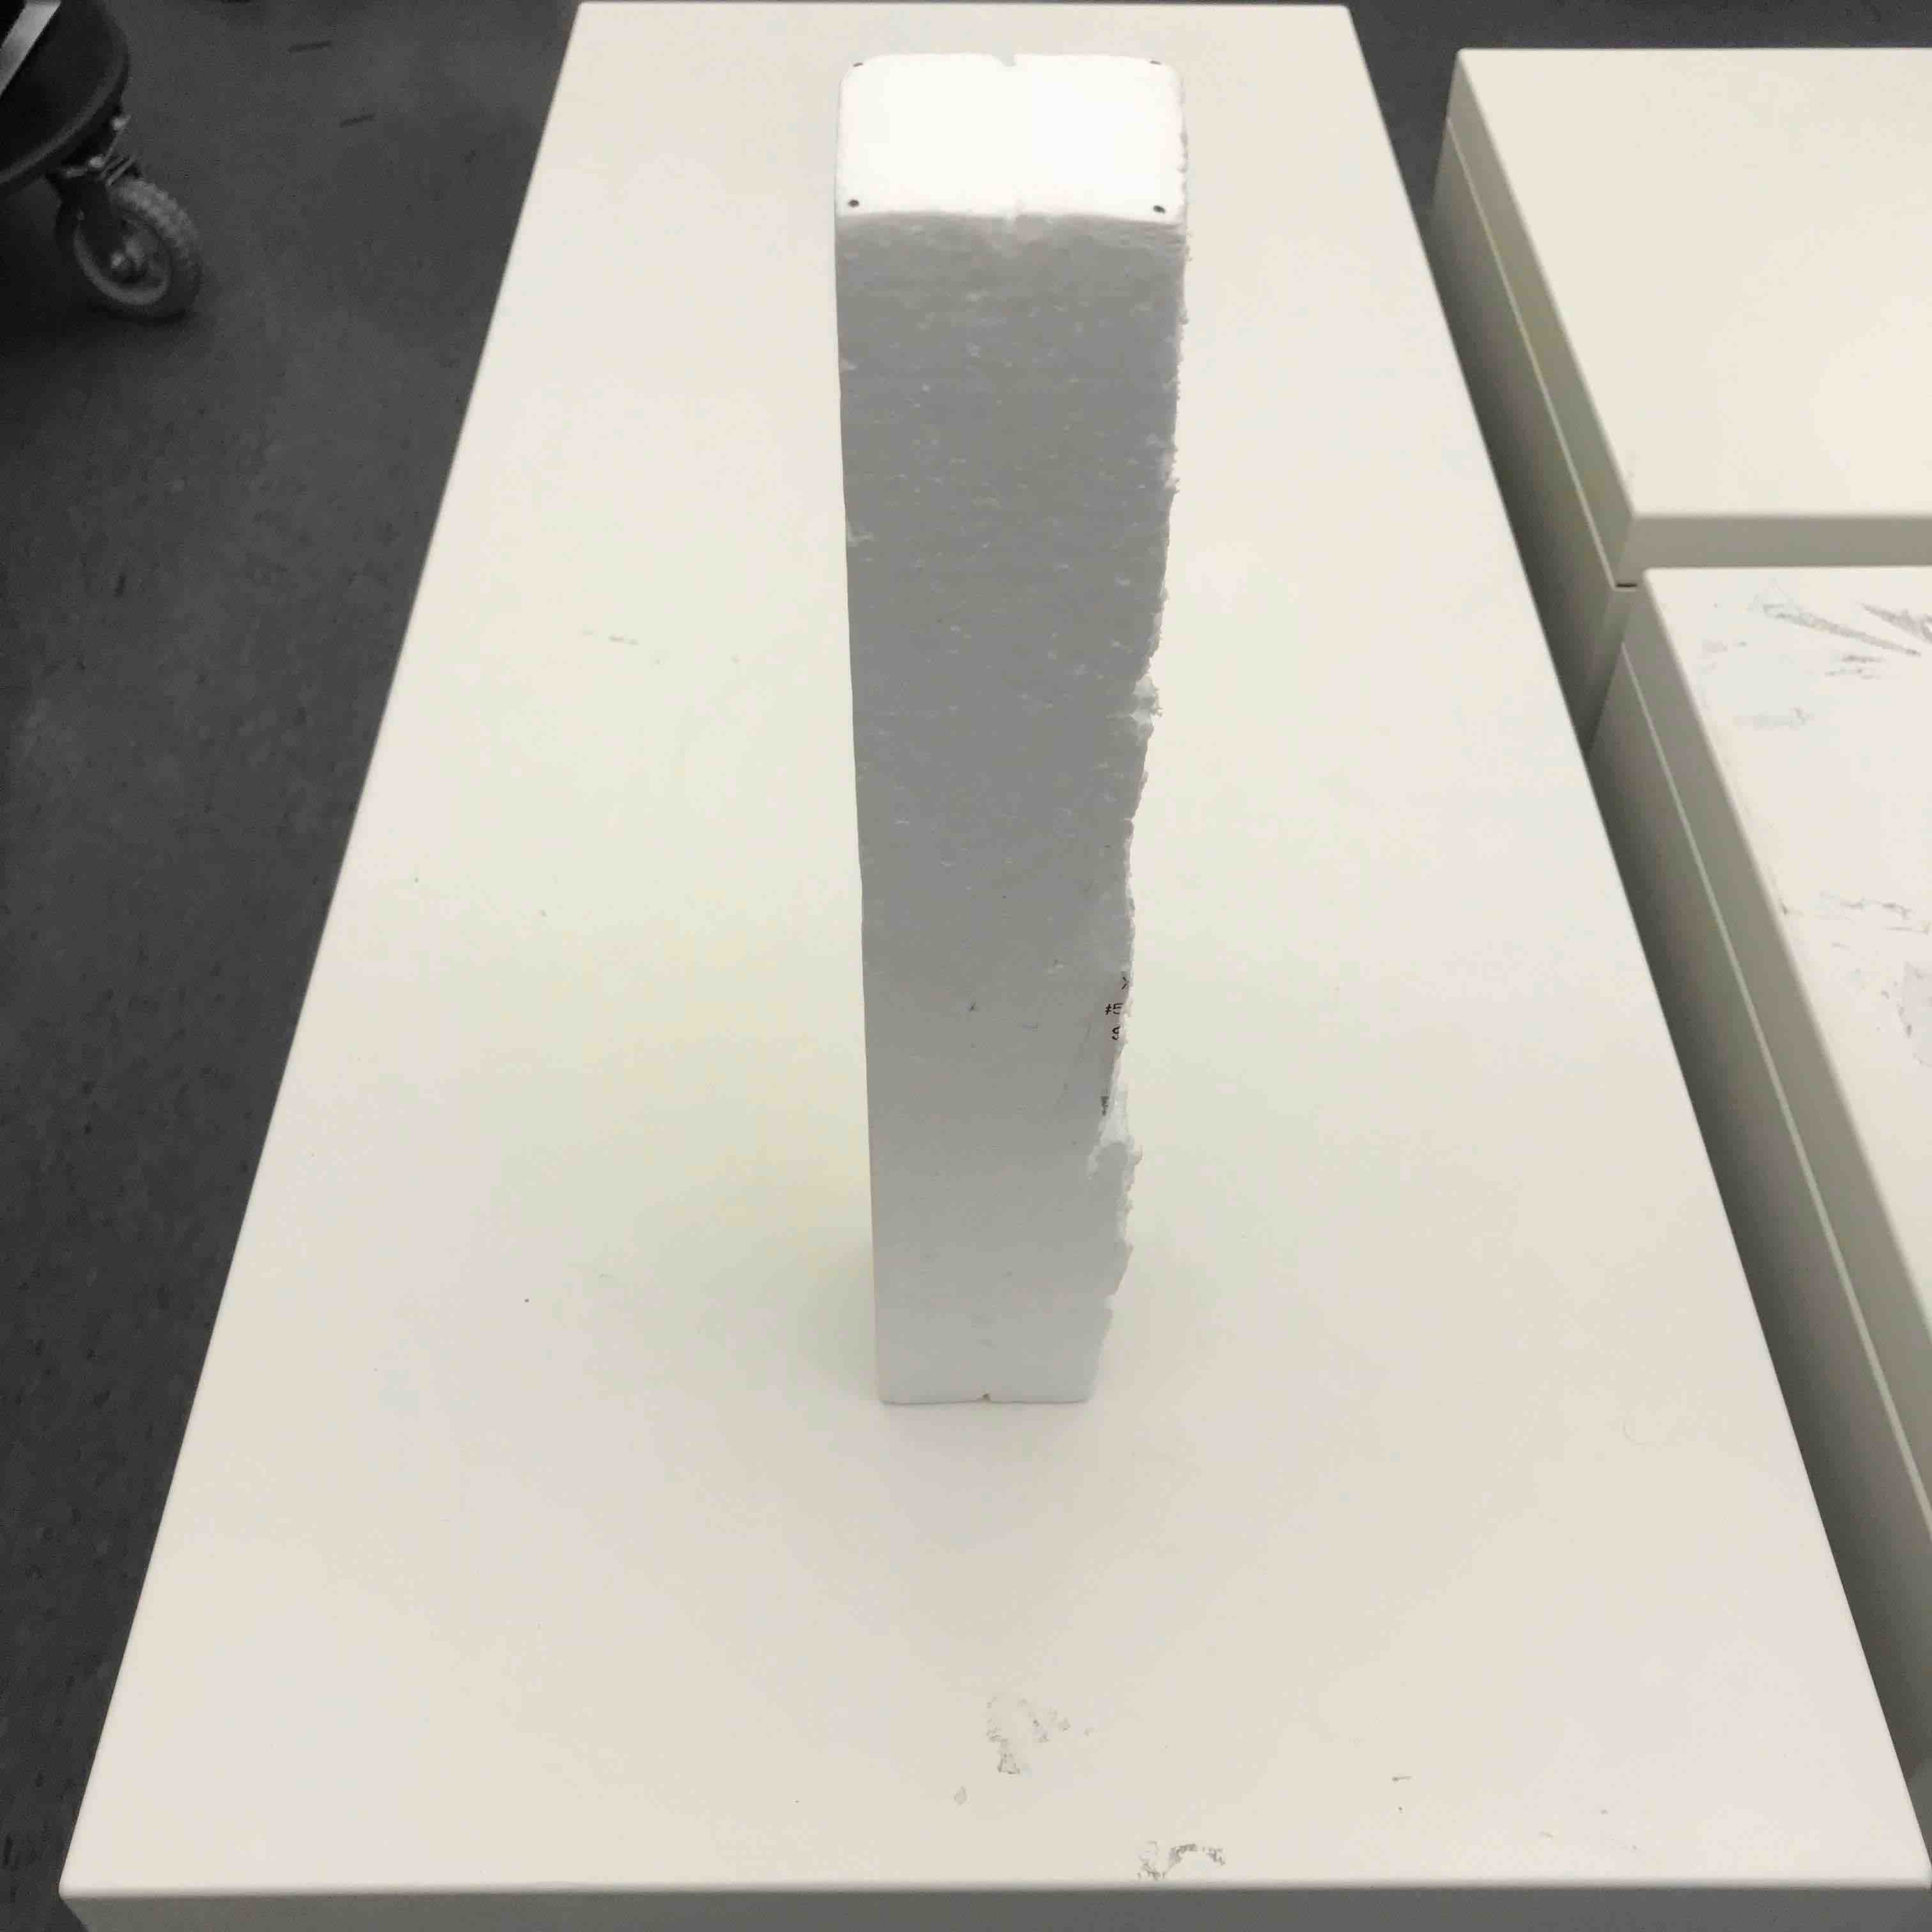
\includegraphics[width=0.3\linewidth]{figures/oidx_28.jpg} \\
  0.03 & 0 \\
\end{tabular}
\end{figure}
Confidence distribution for the \emph{can} concept model on the unseen test set objects after training.
In total, the agent learned 25 new concept models, as well as synonym words for existing concepts, during training.

\begin{figure}
\centering
  
\includegraphics[width=0.7\linewidth]{QR.png}
\end{figure}

}
\end{block}

\end{column}	%%% END COLUMN 3 %%%

%%%%%%%%%%%%%%%%%%%%%%%%%%%%%%%%%%%%%%%%%%%%%%%%%%%%%%%%%%%%%%%%%%%%%%%%%%%%%%%%%%%%%%%%%%%%%%%%%%%%
\end{columns}

\end{frame}

\end{document}


%%%%%%%%%%%%%%%%%%%%%%%%%%%%%%%%%%%%%%%%%%%%%%%%%%%%%%%%%%%%%%%%%%%%%%%%%%%%%%%%%%%%%%%%%%%%%%%%%%%%
%%% Local Variables: 
%%% mode: latex
%%% TeX-PDF-mode: t

